
\section{Experimental verification of Reactive Collision Avoidance}
The Stack of Tasks (SoT) controller with collision avoidance constraints has also been deployed and tested for achieving different postures on the setup in Fig. \ref{fig:TUDSetup}. We have integrated the behavior to path following with the reactive collision avoidance as shown in Fig. \ref{fig:dca}. Though it is integrated, we consider these presented results preliminary yet quite convincing to be go in this direction to develop a reactive collision avoidance technology.

\subsection{Experiments in a mobile robot - PR2{\color{red}  (to be updated)}}

The framework was very initially tested with the given skin cell prototype on PR2, a mobile robot. The skin patch with eight cells is stuck on the arm to sense proximity range information. A simple manipulation scenario is executed and getting close to the arm sensors induced base motion to avoid obstacles while still executing the trajectory. The experiment can be seen here in this \href{https://youtu.be/y-6Oyi21ioQ}{\textcolor{blue}{video}} and the snapshots are shown in this Fig \ref{fig:pr2avoid}. The graph \ref{fig:basegraph} shows the evolution of the robot base when it encounters an obstacle. The safe region is where the skin cell - obstacle distance is within the right limits ensuring safety. Although the base goes away from the obstacle, it recovers back to its previous or commanded pose in the trajectory. 
\begin{figure}[ht]
\centering
\begin{subfigure}
[Getting close to the arm]{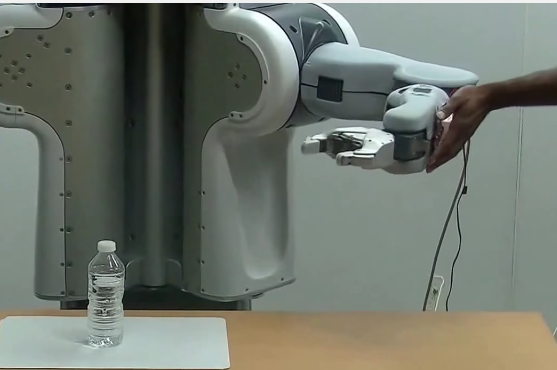
\includegraphics[width=5.5cm,height=6cm]{chapters/doa/images/pr2_0.png}}
\end{subfigure}
\begin{subfigure}
[Base motion to avoid the obstacle]{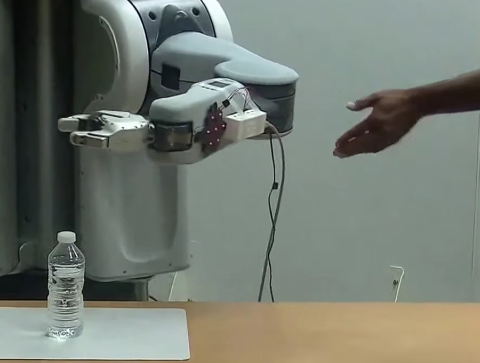
\includegraphics[width=5.5cm,height=6cm]{chapters/doa/images/pr2_1.png}}
\end{subfigure}
\caption{Obstacle Avoidance in PR2 using skin prototype}
\label{fig:pr2avoid}
\end{figure}

\begin{figure}[!ht]
\centering
{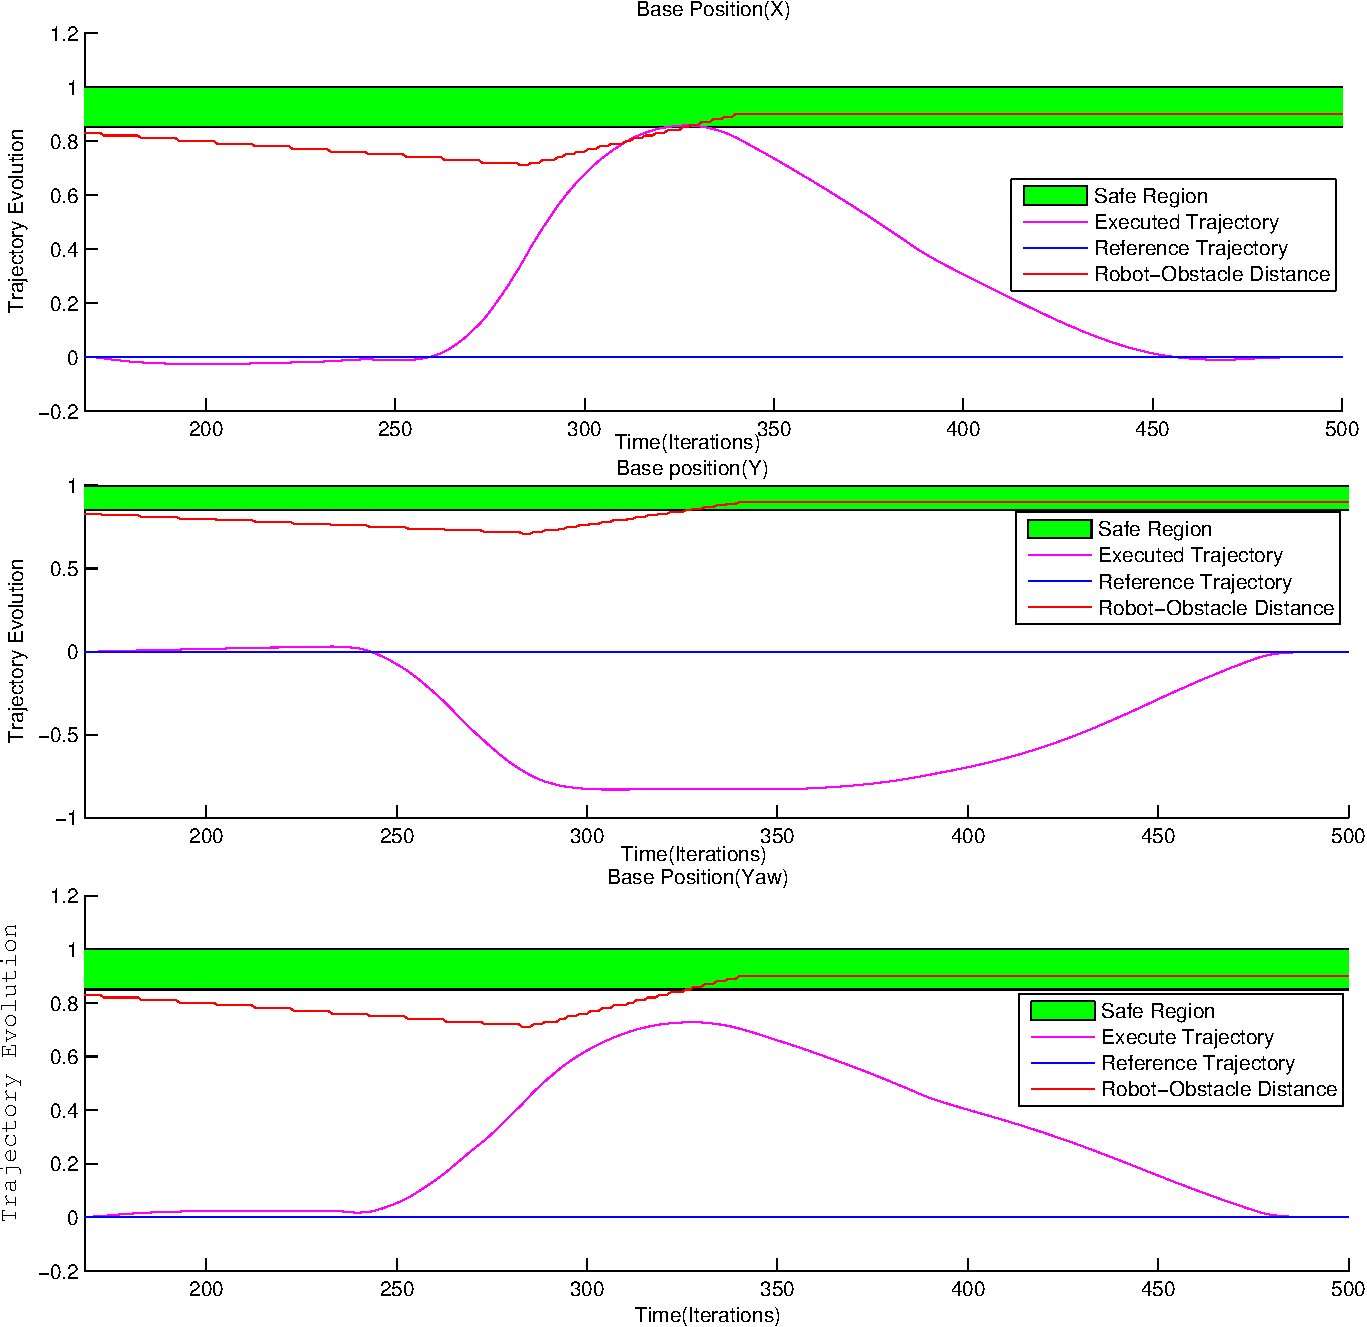
\includegraphics[scale=0.5]{chapters/doa/images/baseplot-crop.pdf}}
\caption{Base Position Evolution}
\label{fig:basegraph}
\end{figure}




\subsection{Experiments with Reactive Replanning in TOMM Setup}
\hypersetup{colorlinks, linkcolor=blue}
The integration of all the components described earlier has been evaluated on a simulation of the orange sorting setup as shown in Fig. \ref{fig:TOMMSimulation}. The evaluation is done in a ROS based gazebo environment with the skin sensors simulated using the flexible collision library to project the distance between objects to sensor range measurements. These measurements are mapped to signals compatible in dynamic graph framework using a bridge component to allow its use in the SoT controller. The reactive planning component having the capability to plan with point cloud data using a Moveit python interface to query motion plan requests. 
\begin{figure}[ht]
\centering
\resizebox{0.85\columnwidth}{!}{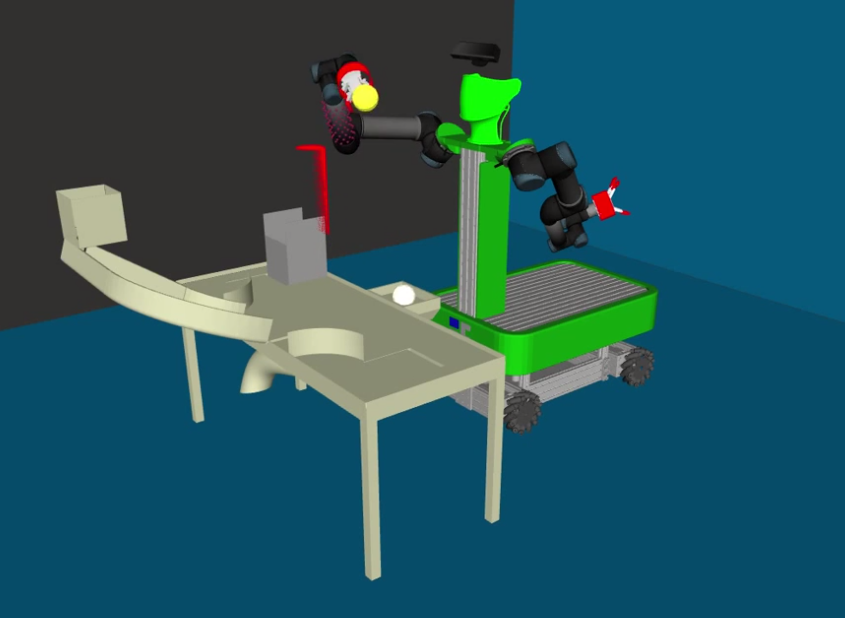
\includegraphics{chapters/doa/images/tomm_simulation.png}}\\[-10pt]
\caption[]{Orange sorting scenario in simulation.}
\label{fig:TOMMSimulation}
\end{figure}
The combined use of a reactive motion planner and a hierarchical reactive SoT controller with skin data makes it a good candidate for applying dynamical obstacle avoidance in factory environments. A video result of the same is available \href{https://youtu.be/uLStjR7mpOI}{\textcolor{blue}{here}}. Though it is tested in simulation, an experimental verification on a real robot setup with 3d cameras is quite essential to qualify the proposed framework as a promising technology. But the collision avoidance is tested on a UR robot with skin sensors to verify the local reactivity of the controller. 

\subsection{Experiments in a UR5 robot}
\begin{figure}[H]
\centering
{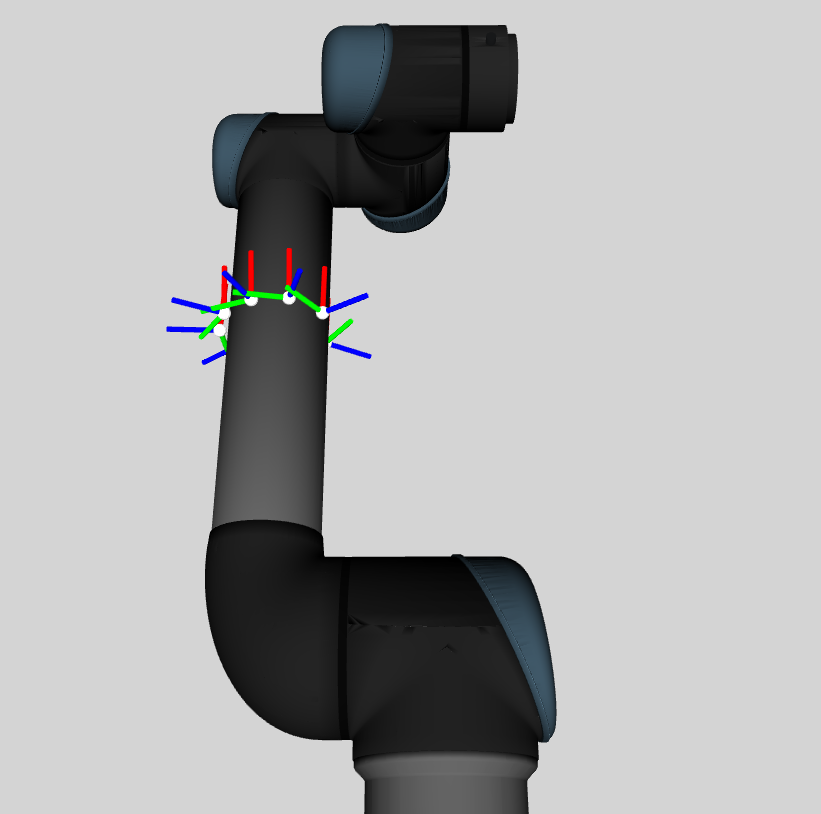
\includegraphics[width=6.5cm,height=6cm]{chapters/doa/images/delft/ring_sensors.png}}
\caption{Sensor Ring on the Upper Arm}
\label{fig:ringsensors}
\end{figure}
The reactive collision avoidance is experimentally verified on the UR5 robot with the skin sensor setup. The skin sensor network  consists of approximately 300 cells in total covering the entire surface of the UR5 robot arm. Though it is interesting to model all the skin cell constraints to be resolved by the controller, it is practically impossible to solve all the inequality constraints using the current state of the art solver due to computational constraints. A proper approximation is necessary to minimize the number of inequality constraints fed to the solver at every control cycle. In the set of preliminary experiments conducted, we defined a skin sensor ring in the upper arm as shown the figure \ref{fig:ringsensors} and collision avoidance constraints are applied only on this ring. The ring's central location on the arm gives symmetry which allows to sense information from all the directions. Another note is that the reactive replanning component is not tested in these experiments because of practical unavailability of the physical setup. 

Predefined trajectories are executed for different obstacle positions with and without collision avoidance task to verify the validity of the collision avoidance mechanism implemented. Three robot positions are chosen: Home position, Pick position and Place position. The repetitiveness of these tests on different object locations is to justify the symmetry of the ring and the robustness of the controller. There is also a complete manipulation scenario shown in the end of experiments to illustrate the practical use of the implementation. This component was successfully integrated in the final project demonstration of Factory-in-a-day which ran for more than 20 minutes robustly without any controller failure though it is possible in the most optimization based solvers. The simplicity of the approach and the practical relevance makes it a best candidate for being used in industries. 
\begin{figure}[H]
\centering
\begin{subfigure}
[Home Position]{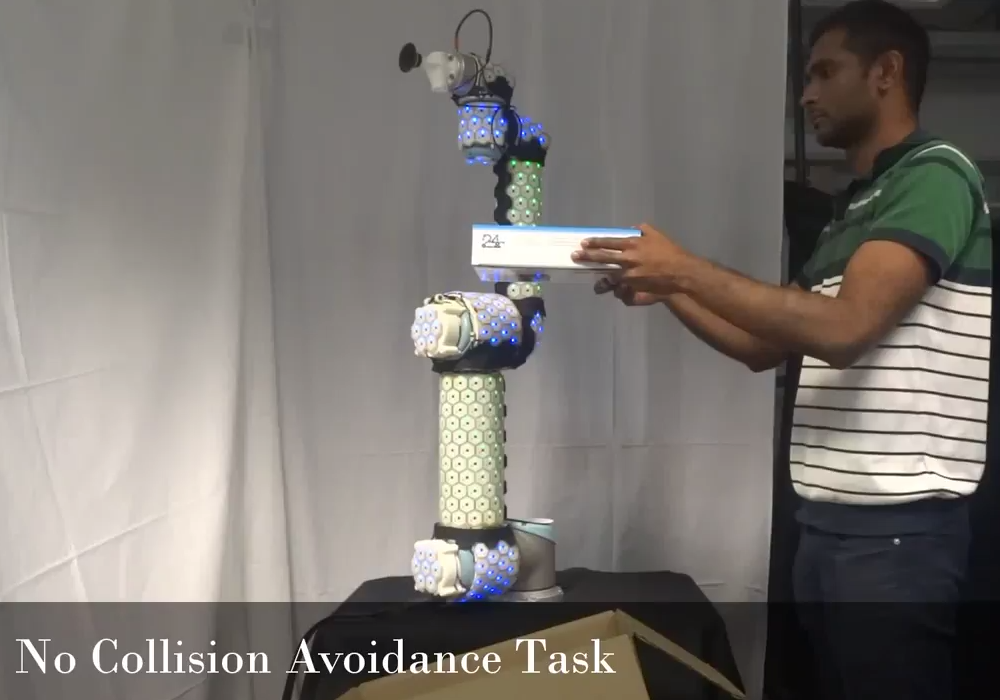
\includegraphics[width=6.5cm,height=6cm]{chapters/doa/images/delft/test_home2pick/cropped/test0_0-cropped.png}}
\end{subfigure}
\begin{subfigure}
[Colliding with Obstacle]{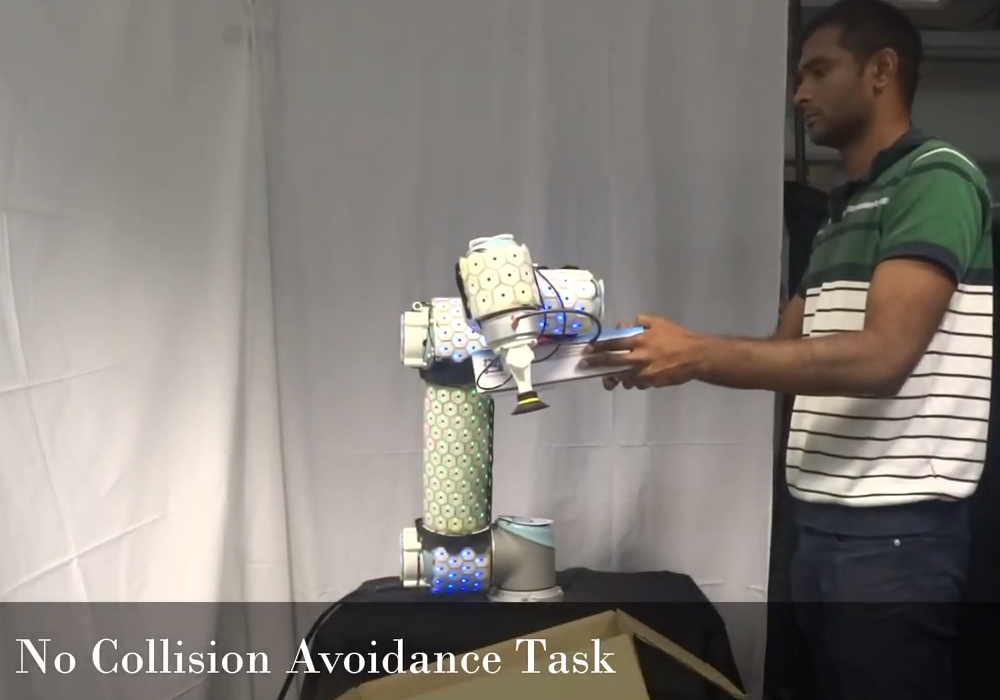
\includegraphics[width=6.5cm,height=6cm]{chapters/doa/images/delft/test_home2pick/cropped/test0_1-cropped.png}}
\end{subfigure}
\begin{subfigure}
[Avoiding Local Collisions]{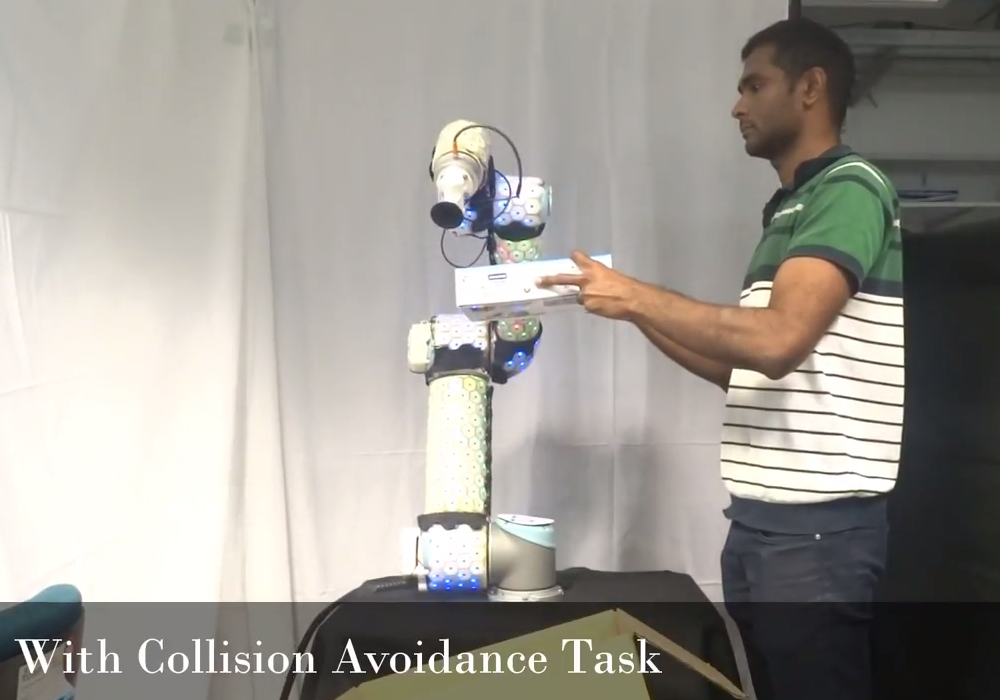
\includegraphics[width=6.5cm,height=6cm]{chapters/doa/images/delft/test_home2pick/cropped/test0_2-cropped.png}}
\end{subfigure}
\begin{subfigure}
[Place Position after avoiding Collisions]{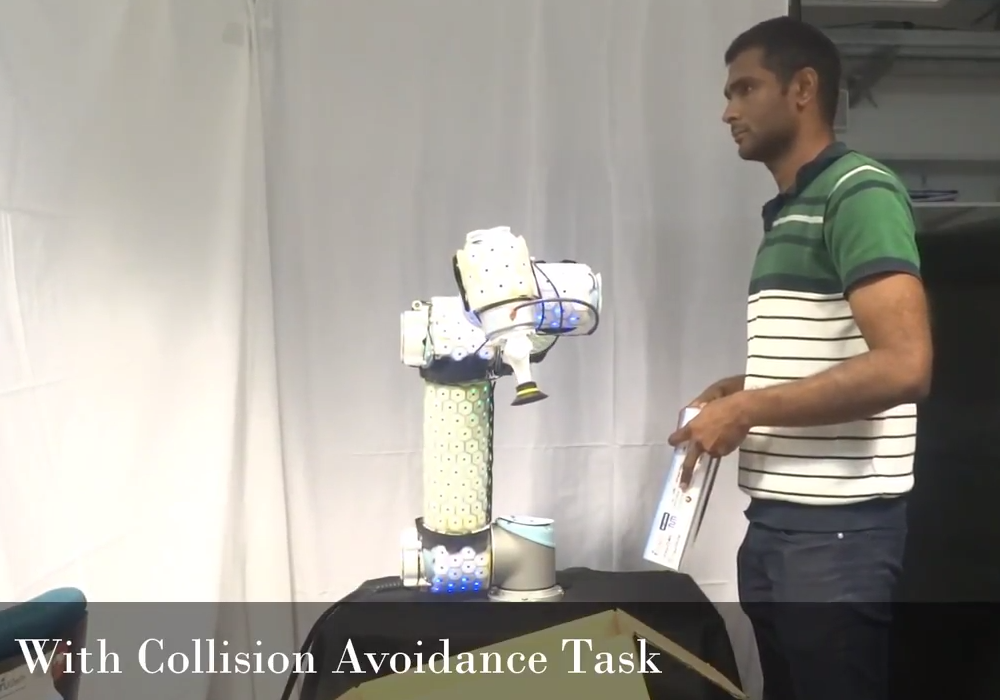
\includegraphics[width=6.5cm,height=6cm]{chapters/doa/images/delft/test_home2pick/cropped/test0_3-cropped.png}}
\end{subfigure}
\caption{Home to Pick Location: Test 1}
\label{fig:h2ptest1}
\end{figure}

\begin{figure}[H]
\centering
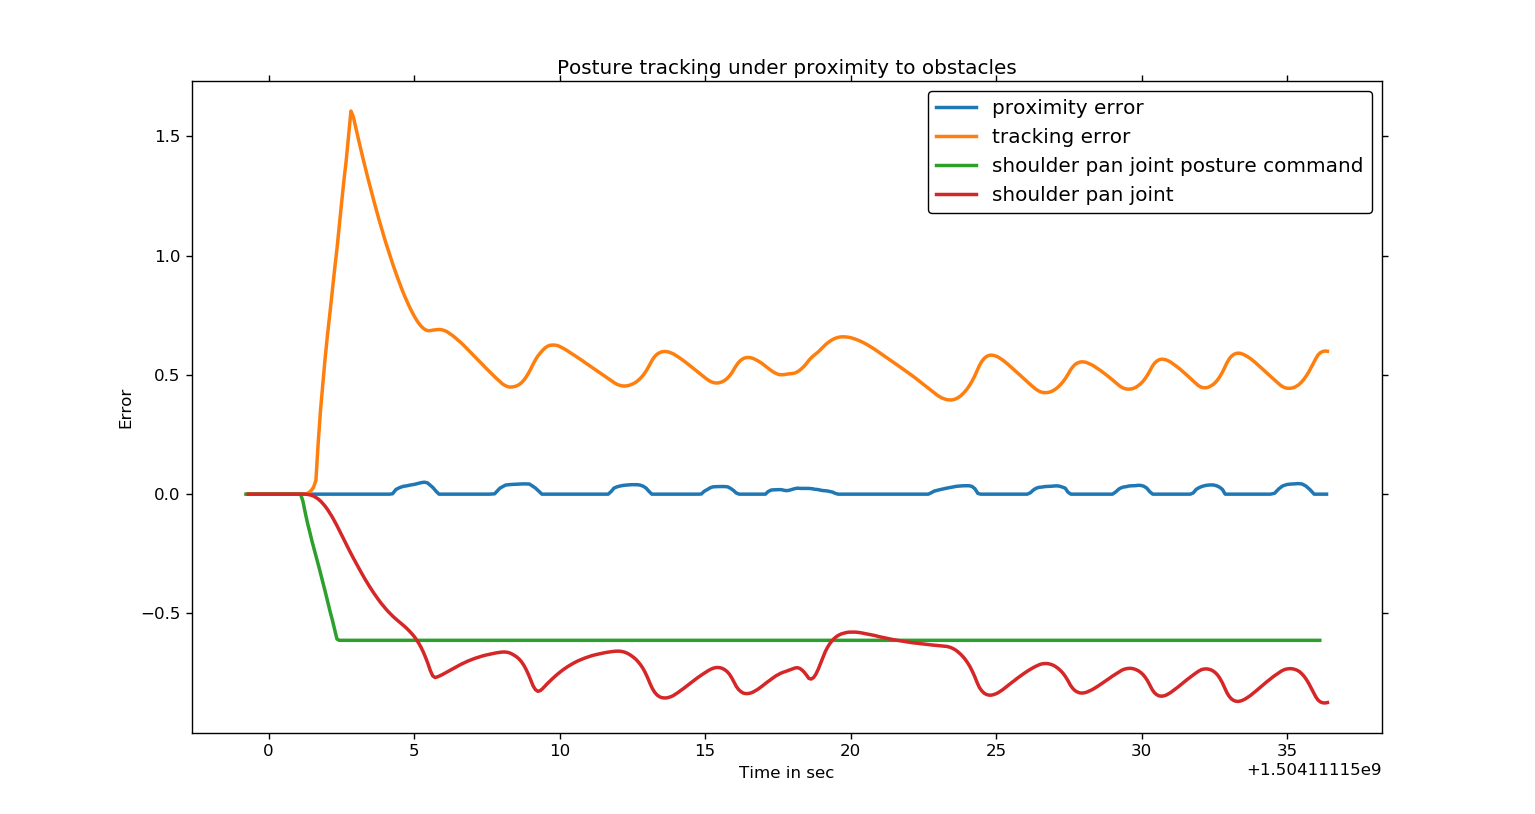
\includegraphics[width=15cm,height=6cm,center]{chapters/doa/images/delft/test_home2pick/test_0.png}
\caption{Home2Pick: Posture/Proximity Error Evolution for Test 1}
\label{Home2Pick:test0}
\end{figure}

\begin{figure}[H]
\centering
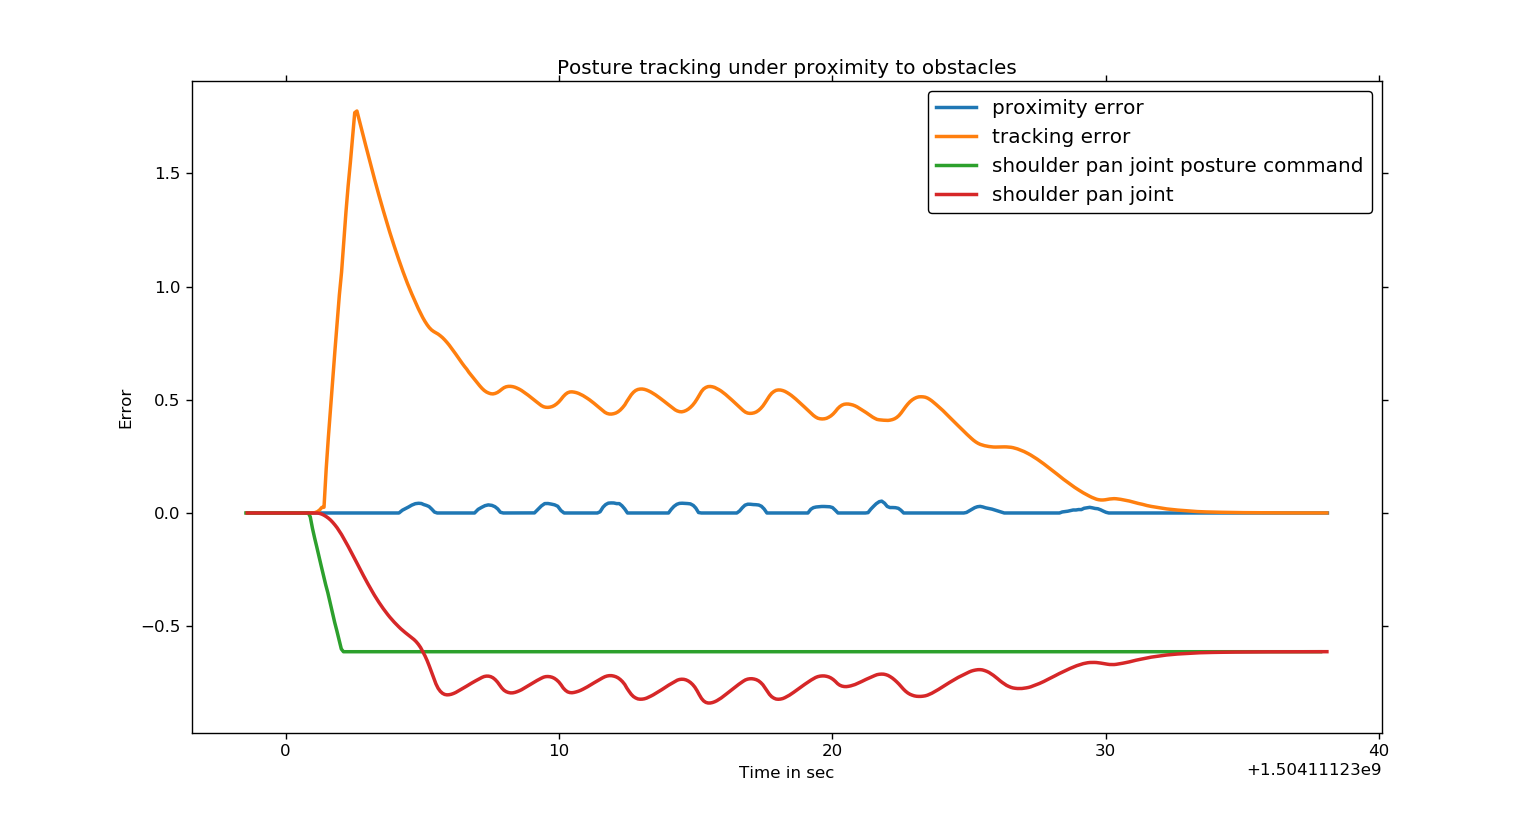
\includegraphics[width=15cm,height=6cm,center]{chapters/doa/images/delft/test_home2pick/test_1.png}
\caption{Home2Pick: Posture/Proximity Error Evolution for Test 2}
\label{Home2Pick:test1}
\end{figure}
\begin{figure}[H]
\centering
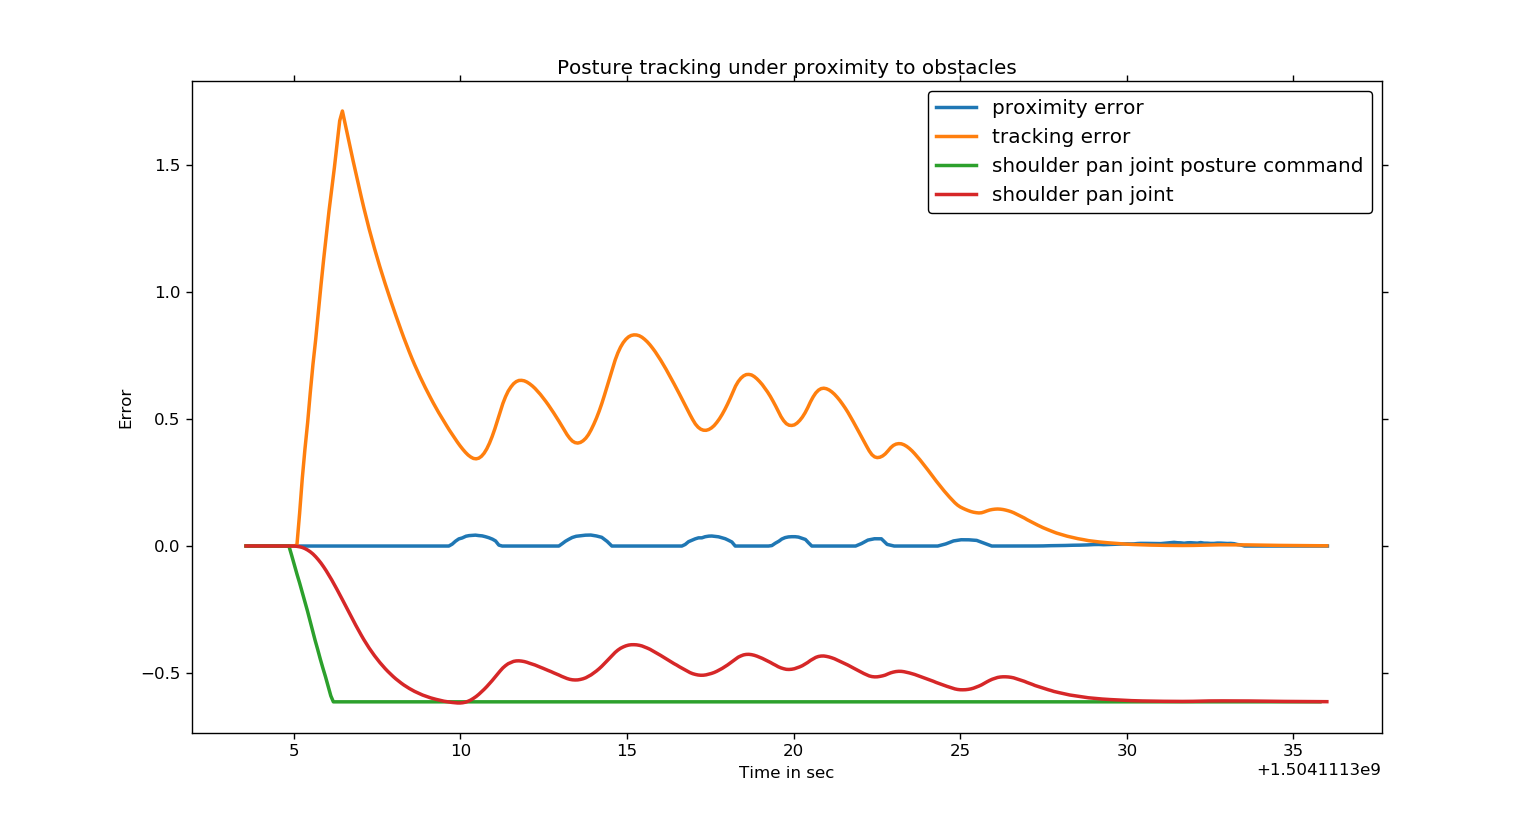
\includegraphics[width=15cm,height=6cm,center]{chapters/doa/images/delft/test_home2pick/test_2.png}
\caption{Home2Pick: Posture/Proximity Error Evolution for Test 3}
\label{Home2Pick:test2}
\end{figure}
\subsubsection{Home to Pick}
\begin{figure}[H]
\centering
\begin{subfigure}
[Home Position]{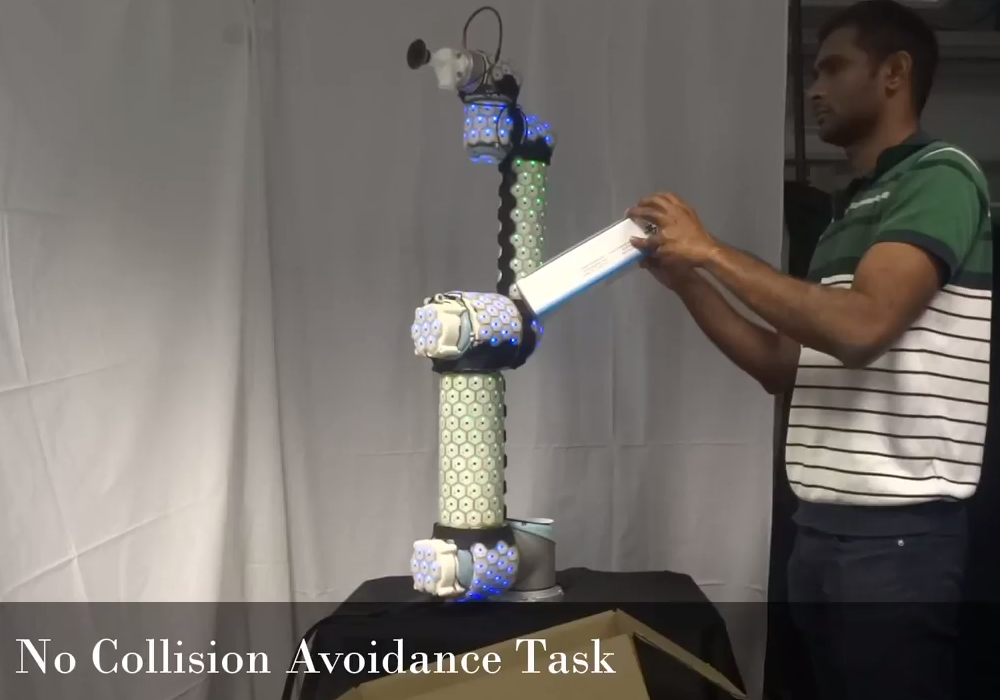
\includegraphics[width=6.5cm,height=6cm]{chapters/doa/images/delft/test_home2pick/cropped/test1_0-cropped.png}}
\end{subfigure}
\begin{subfigure}
[Colliding with Obstacle]{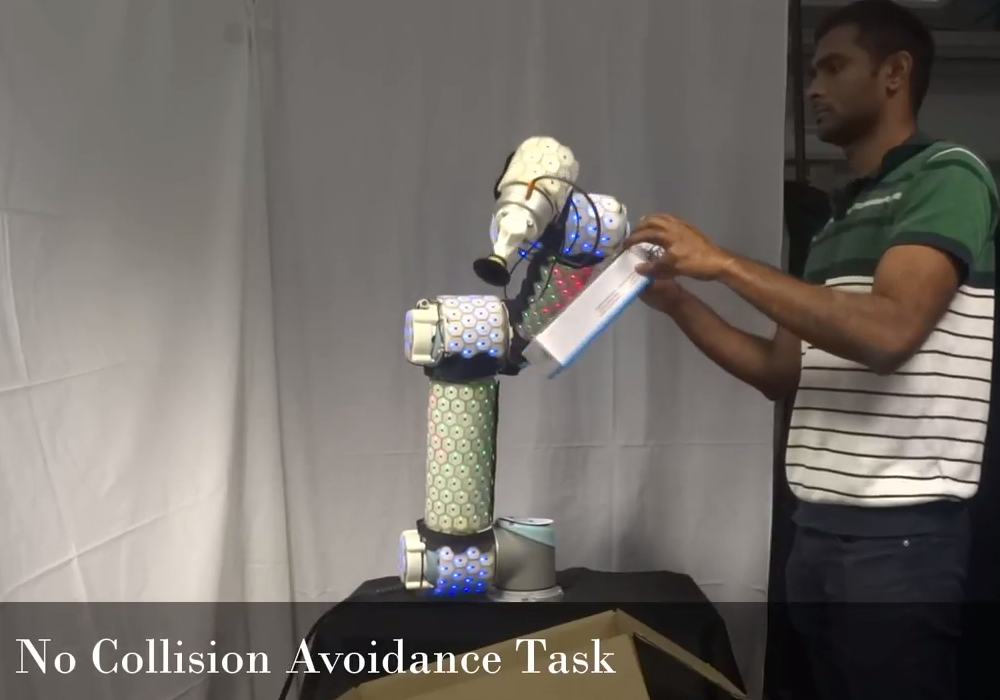
\includegraphics[width=6.5cm,height=6cm]{chapters/doa/images/delft/test_home2pick/cropped/test1_1-cropped.png}}
\end{subfigure}
\begin{subfigure}
[Avoiding Local Collisions]{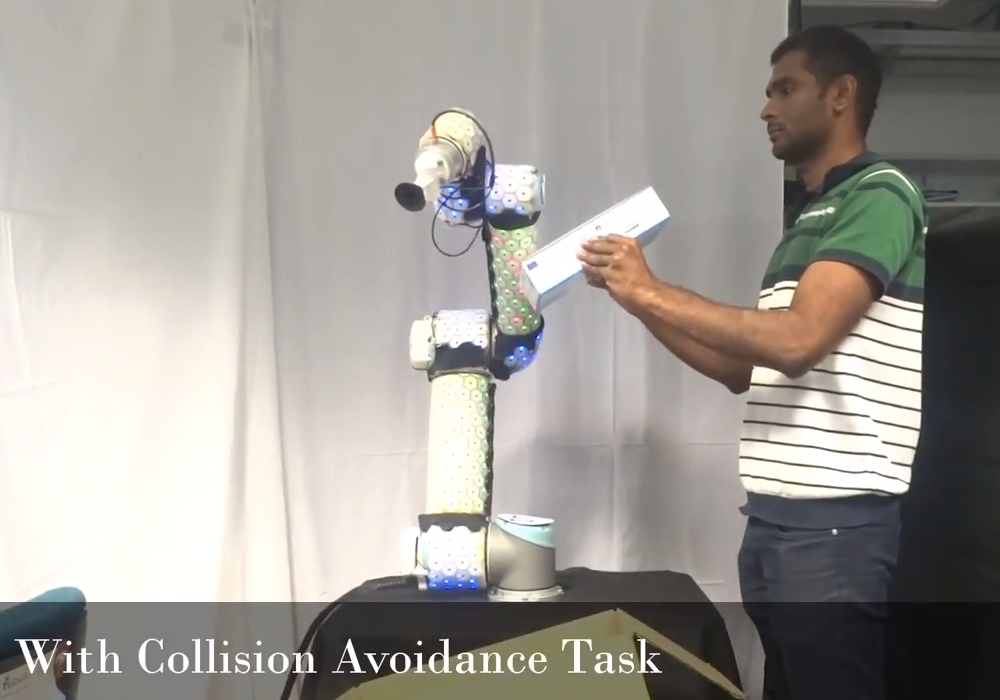
\includegraphics[width=6.5cm,height=6cm]{chapters/doa/images/delft/test_home2pick/cropped/test1_2-cropped.png}}
\end{subfigure}
\begin{subfigure}
[Place Position after avoiding Collisions]{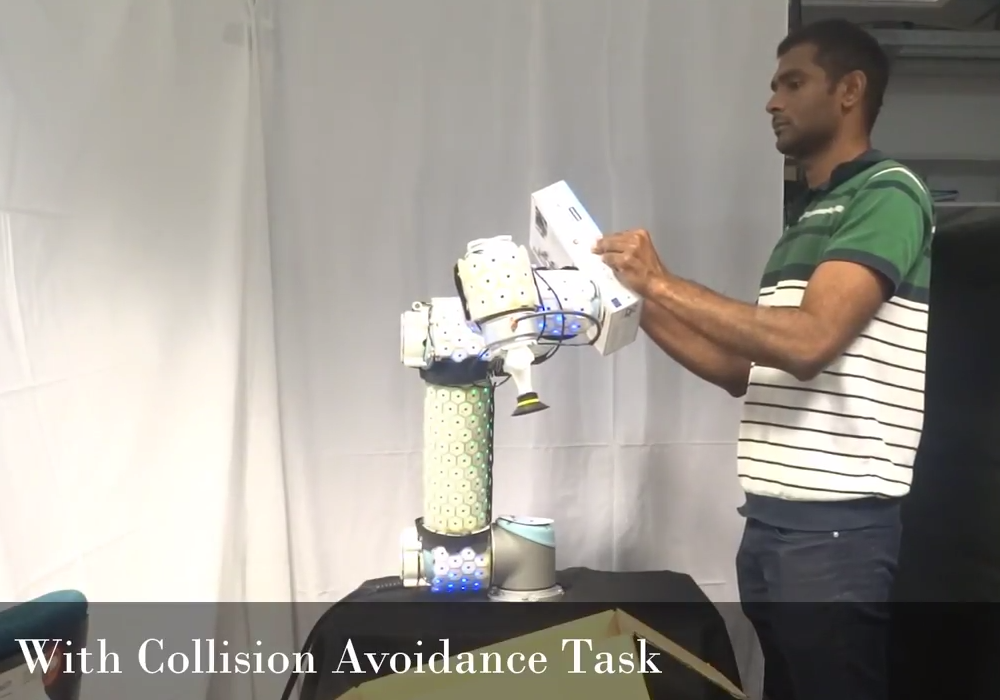
\includegraphics[width=6.5cm,height=6cm]{chapters/doa/images/delft/test_home2pick/cropped/test1_3-cropped.png}}
\end{subfigure}
\caption{Home to Pick Location: Test 2}
\label{fig:h2ptest2}
\end{figure}

The experimental validation can be seen in this \href{https://goo.gl/LVbQZz}{\textcolor{blue}{home to pick}} video. As it can be seen, a box is used as an obstacle to interrupt the executed path. Three tests are conducted at different obstacle locations introducing variability in goals. The figure \ref{fig:h2ptest1} shows the first test with a fixed obstacle location through out this test. (a) shows the initial state of the robot which is the home position and (b) shows the trajectory execution without any collision avoidance task to differentiate with the behavior  generated by the controller with collision avoidance task. The robot evading collisions and its inability to reach the goal because of the object can be seen in (c) and (d). It gets stuck in local minima but manages to reach the goal after the object is removed. The plot in \ref{Home2Pick:test0}, \ref{Home2Pick:test1}, \ref{Home2Pick:test2} shows the evolution of the trajectory tracking error and the proximity distance error during the execution of test 1 with collision avoidance task. The trajectory tracking error is the 2-norm of the current state of the robot and the posture command of the trajectory sequencer fed to posture task stacked in the solver. The proximity error is the 2-norm of the safety margin and the all the range measurements the skin cells expressing the vicinity of an obstacle to the defined skin cell ring. 

It can be observed in the plot \ref{Home2Pick:test0} that the tracking error oscillates in response to the perturbations in the proximity error which intuitively explains the closeness with the obstacles when executing the trajectory. As we observed in the test 1, the robot gets stuck in local minima which is explained by the non-zero tracking error at the end of the measured cycle. The shoulder pan joint states and posture command are also plotted to justify the behavior. It can be noted there is a peak increase in the tracking error which is due to fast update of the posture command and the conservative gains of the controller though the controller can be tuned to perform faster with the right gains of the collision avoidance task. 


The figure \ref{fig:h2ptest2} shows the second test with a fixed obstacle location through out this test. (a) shows the initial state of the robot which is the home position and (b) shows the trajectory execution without any collision avoidance task to differentiate with the behavior generated by the controller with collision avoidance task. The robot evading collisions and its inability to reach the goal because of the object can be seen in (c) and (d). Just like in the previous test, it hits a local minima but reaches the goal when the obstacle is removed. 

The figure \ref{fig:h2ptest3} shows the third test with a fixed obstacle location through out this test. (a) shows the initial state of the robot which is the home position and (b) shows the trajectory execution without any collision avoidance task to differentiate with the behavior generated by the controller with collision avoidance task. The robot avoiding collisions to reach the final state which can be seen in (c) and (d). A behavior similar to test 1 can be observed in the plots \ref{Home2Pick:test1} and \ref{Home2Pick:test2} though the tracking error finally reaches zero value showing the success in reaching the destination avoiding the collisions.

\begin{figure}[H]
\centering
\begin{subfigure}
[Home Position]{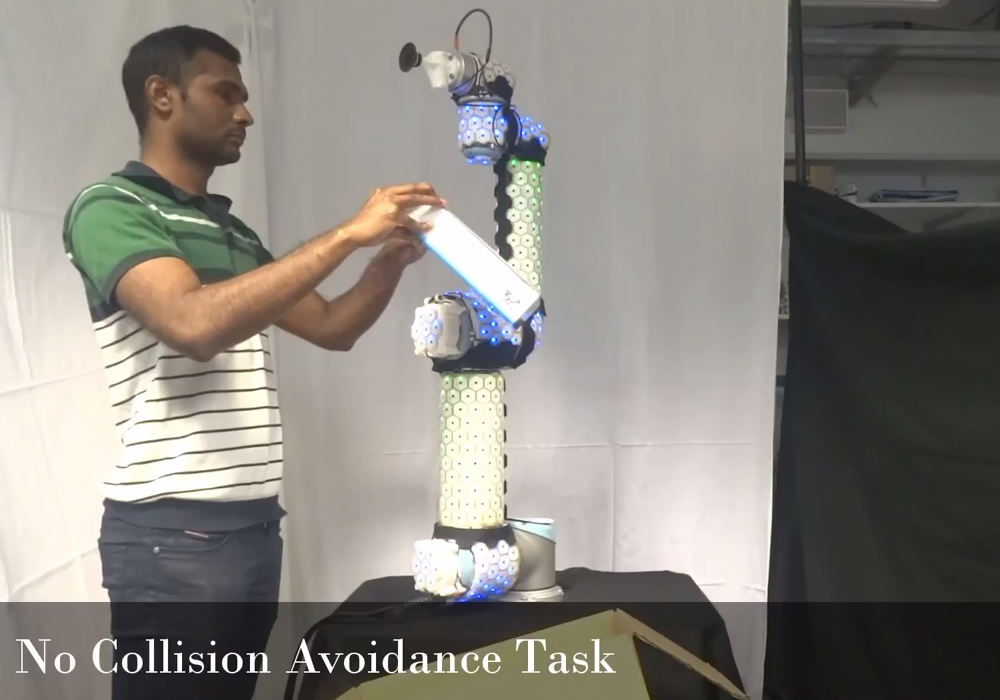
\includegraphics[width=6.5cm,height=6cm]{chapters/doa/images/delft/test_home2pick/cropped/test2_0-cropped.png}}
\end{subfigure}
\begin{subfigure}
[Colliding with Obstacle]{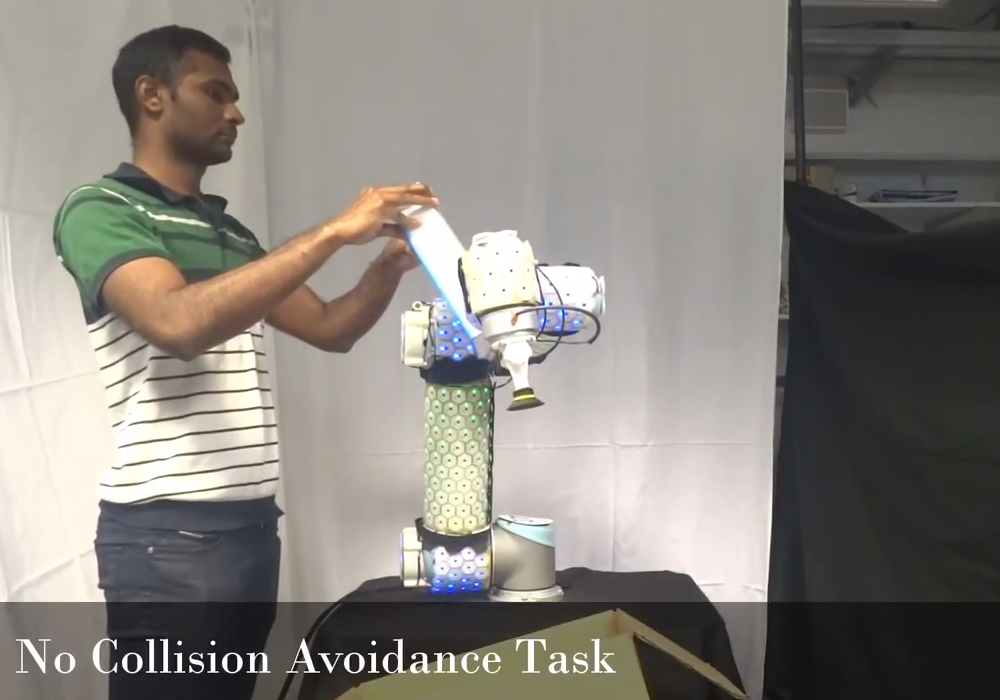
\includegraphics[width=6.5cm,height=6cm]{chapters/doa/images/delft/test_home2pick/cropped/test2_1-cropped.png}}
\end{subfigure}
\begin{subfigure}
[Avoiding Local Collisions]{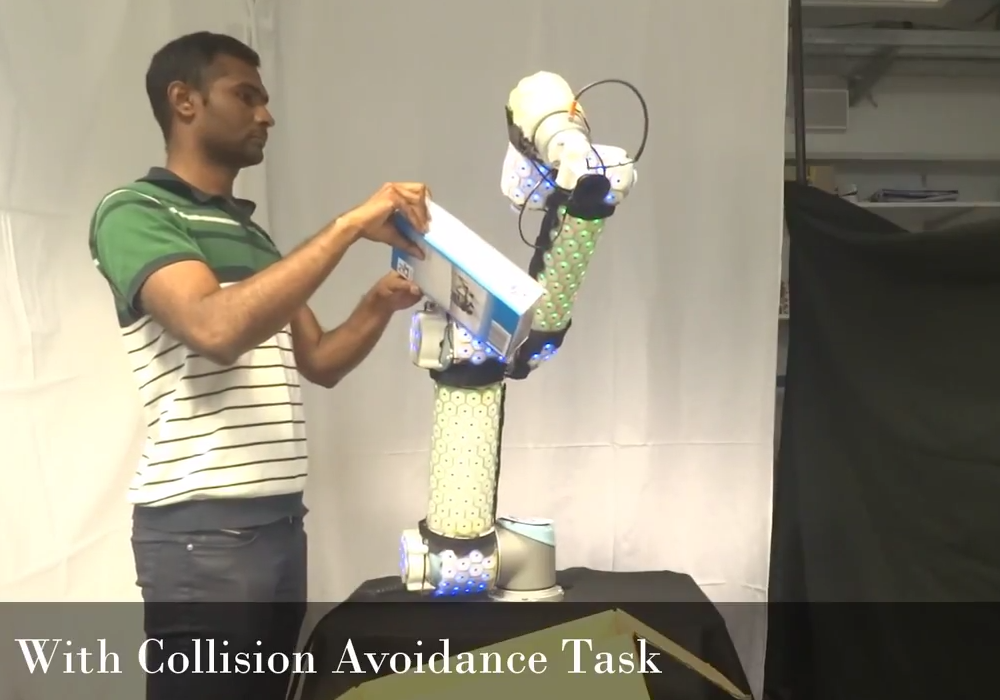
\includegraphics[width=6.5cm,height=6cm]{chapters/doa/images/delft/test_home2pick/cropped/test2_2-cropped.png}}
\end{subfigure}
\begin{subfigure}
[Place Position after avoiding Collisions]{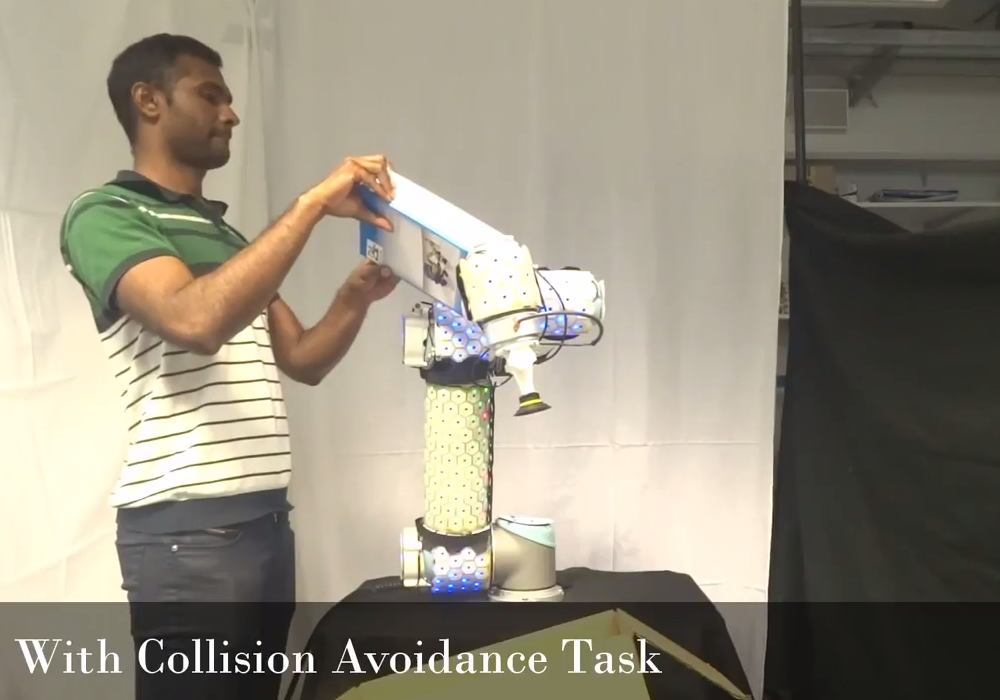
\includegraphics[width=6.5cm,height=6cm]{chapters/doa/images/delft/test_home2pick/cropped/test2_3-cropped.png}}
\end{subfigure}
\caption{Home to Pick Location: Test 3}
\label{fig:h2ptest3}
\end{figure}

\subsubsection{Pick to Place}

The validation can be seen in the \href{https://goo.gl/7jCqzA}{\textcolor{blue}{pick to place}} experiment video. Similar to the previous test, three different obstacle locations are chosen to verify the behavior. The figure \ref{fig:p2ptest1} shows the second test with a fixed obstacle location through out this test. (a) shows the initial state of the robot which is the home position and (b) shows the trajectory execution without any collision avoidance task to differentiate with the behavior generated by the controller with collision avoidance task. The robot evading collisions and its inability to reach the goal because of the object can be seen in (c), (d), (e) and (f). 
\begin{figure}[H]
\centering
\begin{subfigure}
[Home Position]{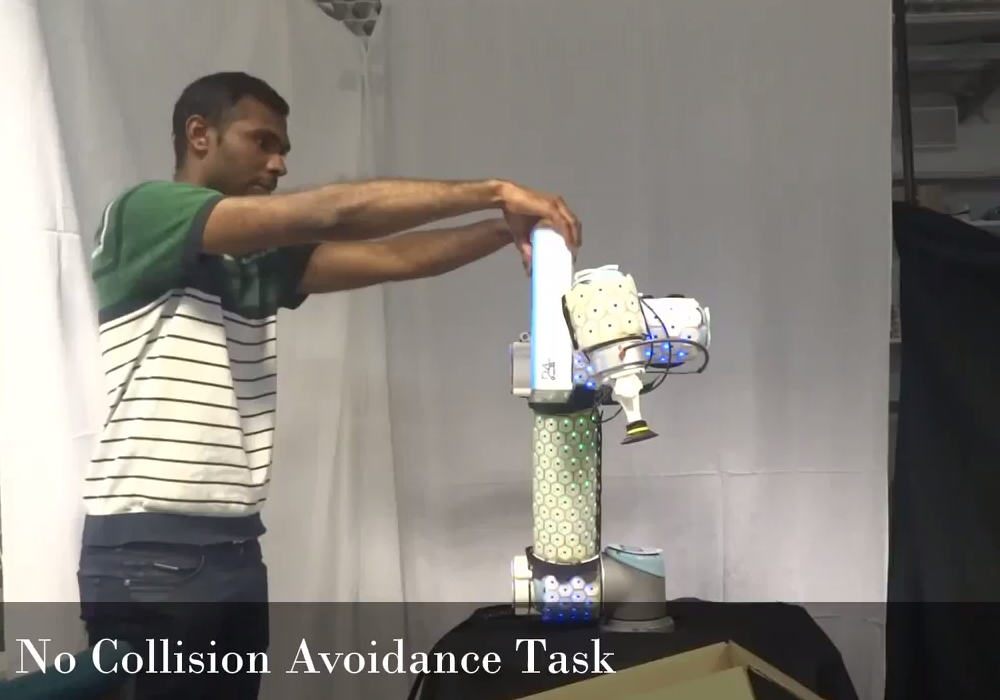
\includegraphics[width=6.5cm,height=6cm]{chapters/doa/images/delft/test_pick2place/cropped/test0_0-cropped.png}}
\end{subfigure}
\begin{subfigure}
[Colliding with Obstacle]{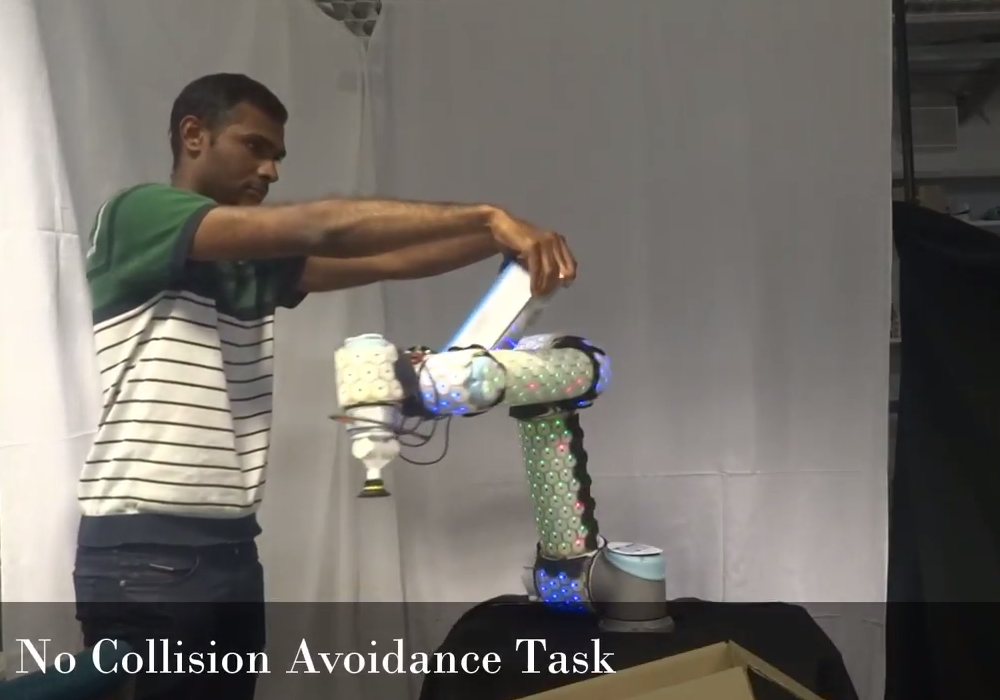
\includegraphics[width=6.5cm,height=6cm]{chapters/doa/images/delft/test_pick2place/cropped/test0_1-cropped.png}}
\end{subfigure}
\begin{subfigure}
[Avoiding Local Collisions 1/3]{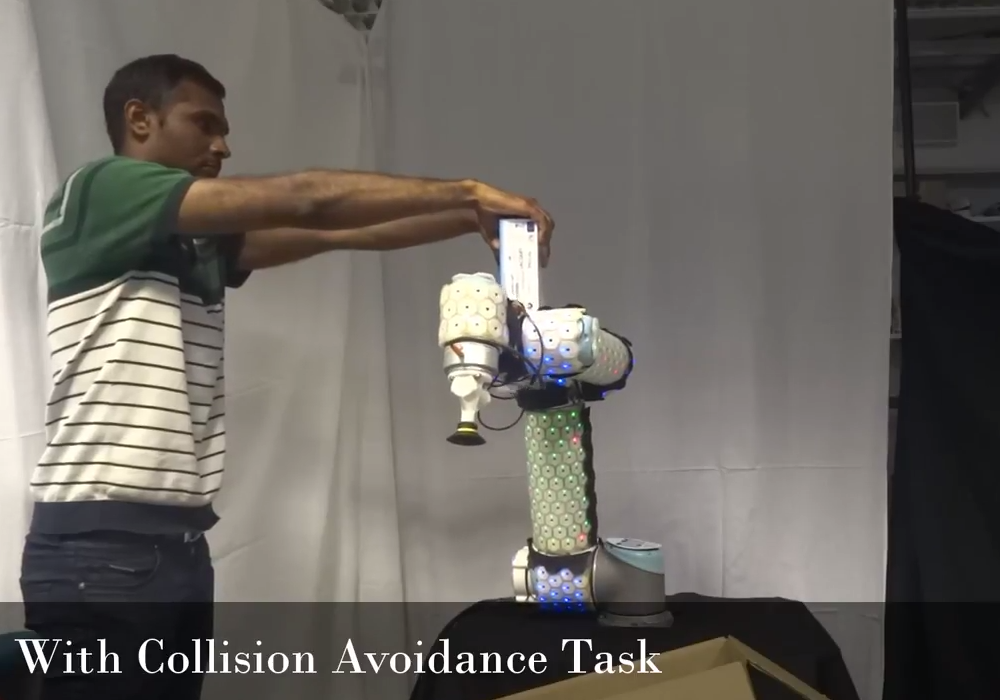
\includegraphics[width=6.5cm,height=6cm]{chapters/doa/images/delft/test_pick2place/cropped/test0_2_0-cropped.png}}
\end{subfigure}
\begin{subfigure}
[Avoiding Local Collisions 2/3]{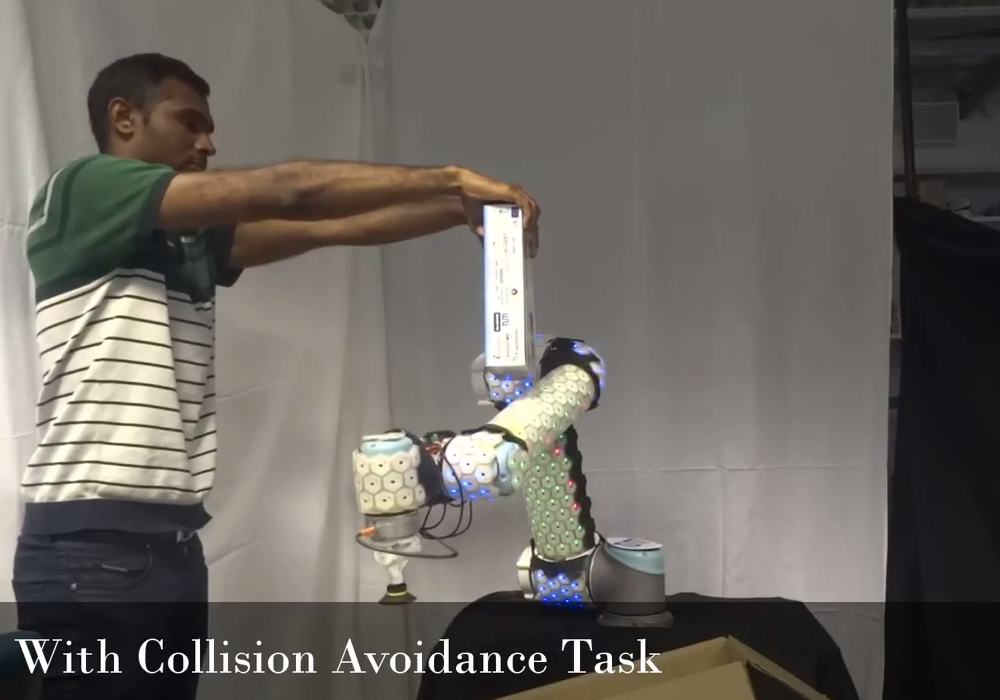
\includegraphics[width=6.5cm,height=6cm]{chapters/doa/images/delft/test_pick2place/cropped/test0_2_1-cropped.png}}
\end{subfigure}
\begin{subfigure}
[Avoiding Local Collisions 3/3]{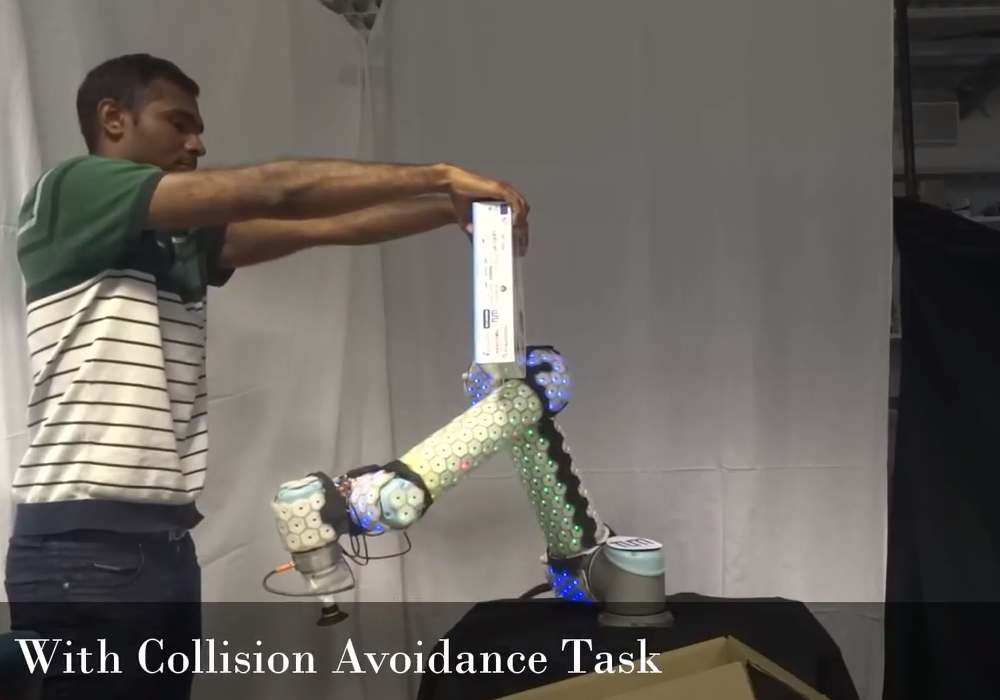
\includegraphics[width=6.5cm,height=6cm]{chapters/doa/images/delft/test_pick2place/cropped/test0_2_2-cropped.png}}
\end{subfigure}
\begin{subfigure}
[Final State - Place Position]{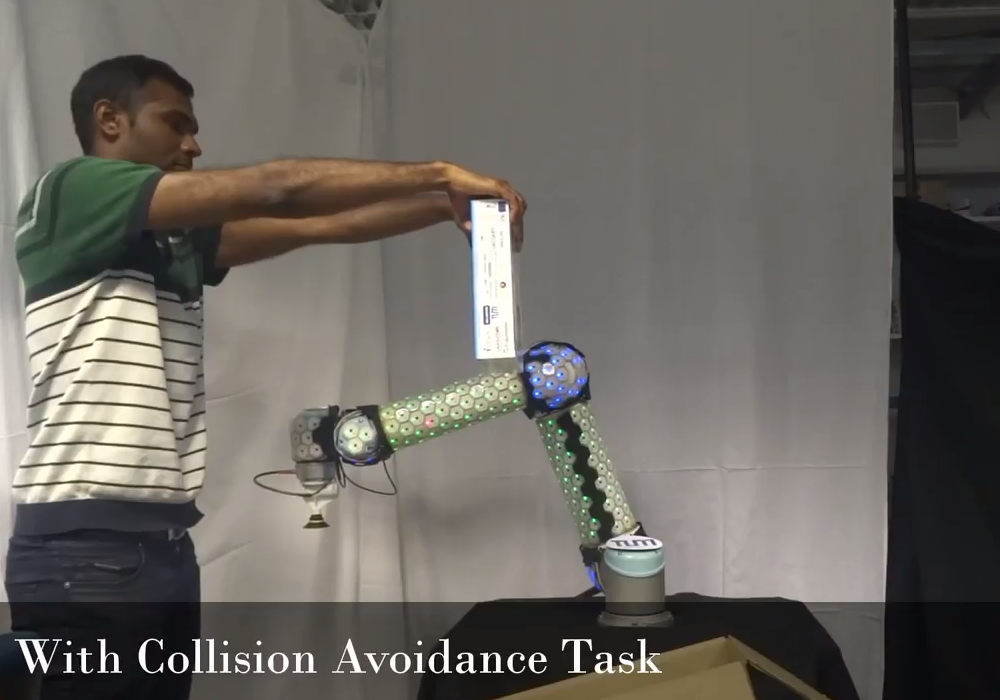
\includegraphics[width=6.5cm,height=6cm]{chapters/doa/images/delft/test_pick2place/cropped/test0_3-cropped.png}}
\end{subfigure}
\caption{Pick to Place Location: Test 1}
\label{fig:p2ptest1}
\end{figure}

\begin{figure}[H]
\centering
\begin{subfigure}
[Initial State - Home Position]{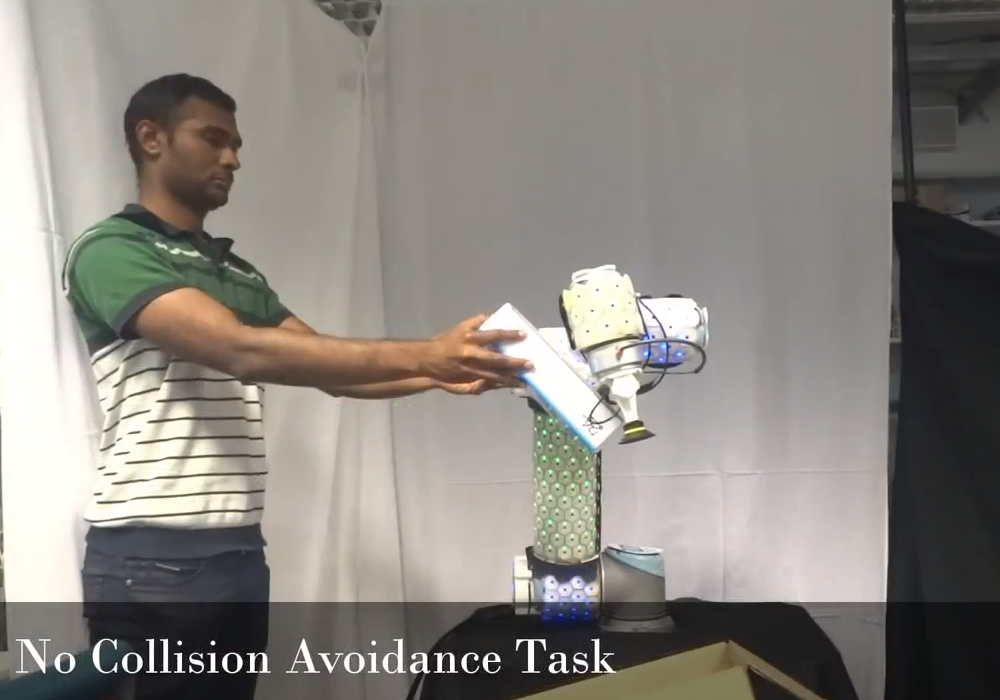
\includegraphics[width=6.5cm,height=6cm]{chapters/doa/images/delft/test_pick2place/cropped/test1_0-cropped.png}}
\end{subfigure}
\begin{subfigure}
[Colliding with Obstacle]{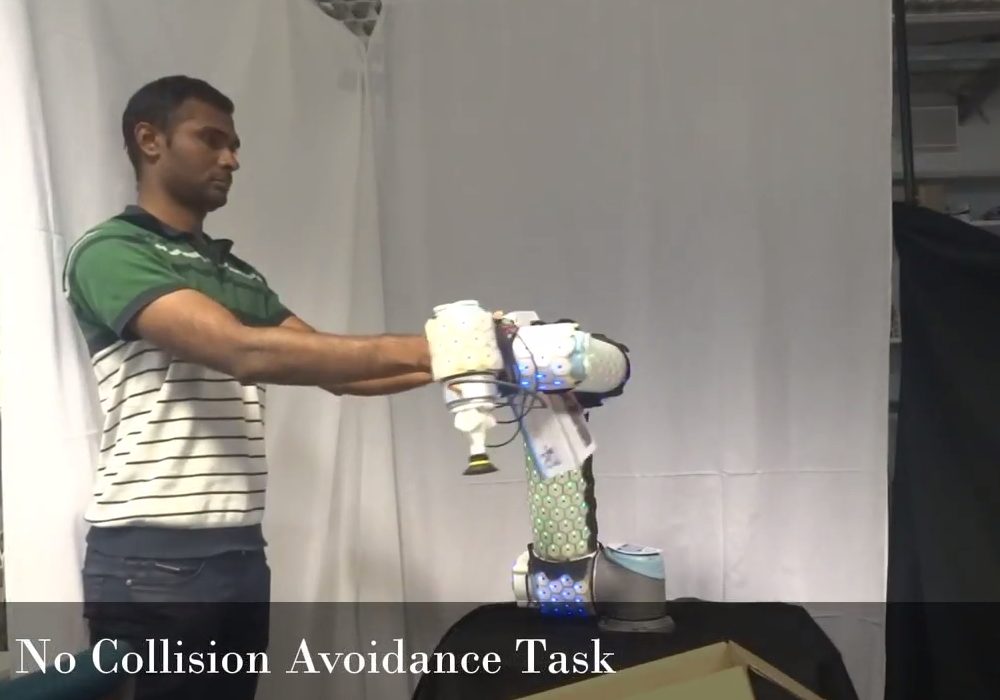
\includegraphics[width=6.5cm,height=6cm]{chapters/doa/images/delft/test_pick2place/cropped/test1_1-cropped.png}}
\end{subfigure}
\begin{subfigure}
[Avoiding Local Collisions 1/3]{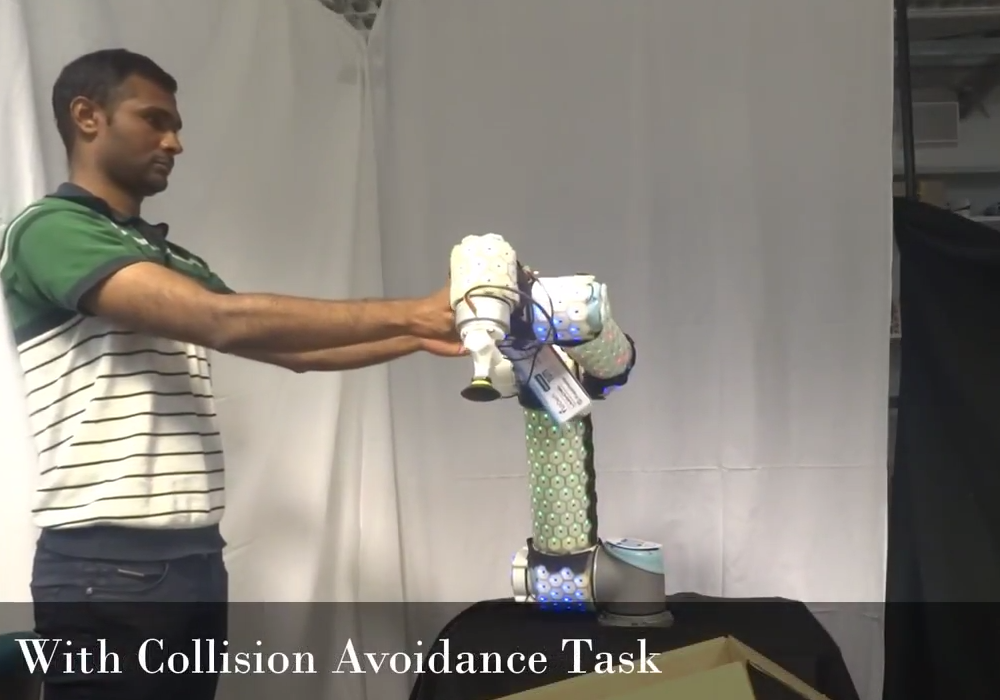
\includegraphics[width=6.5cm,height=6cm]{chapters/doa/images/delft/test_pick2place/cropped/test1_2-cropped.png}}
\end{subfigure}
\begin{subfigure}
[Avoiding Local Collisions 2/3]{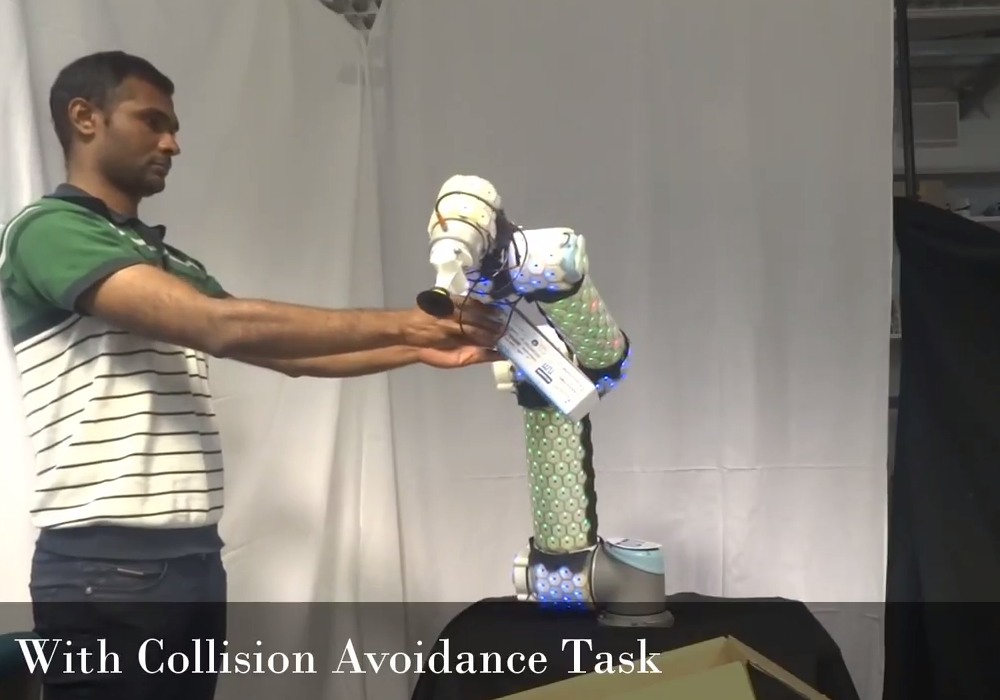
\includegraphics[width=6.5cm,height=6cm]{chapters/doa/images/delft/test_pick2place/cropped/test1_2_1-cropped.png}}
\end{subfigure}
\begin{subfigure}
[Avoiding Local Collisions 3/3]{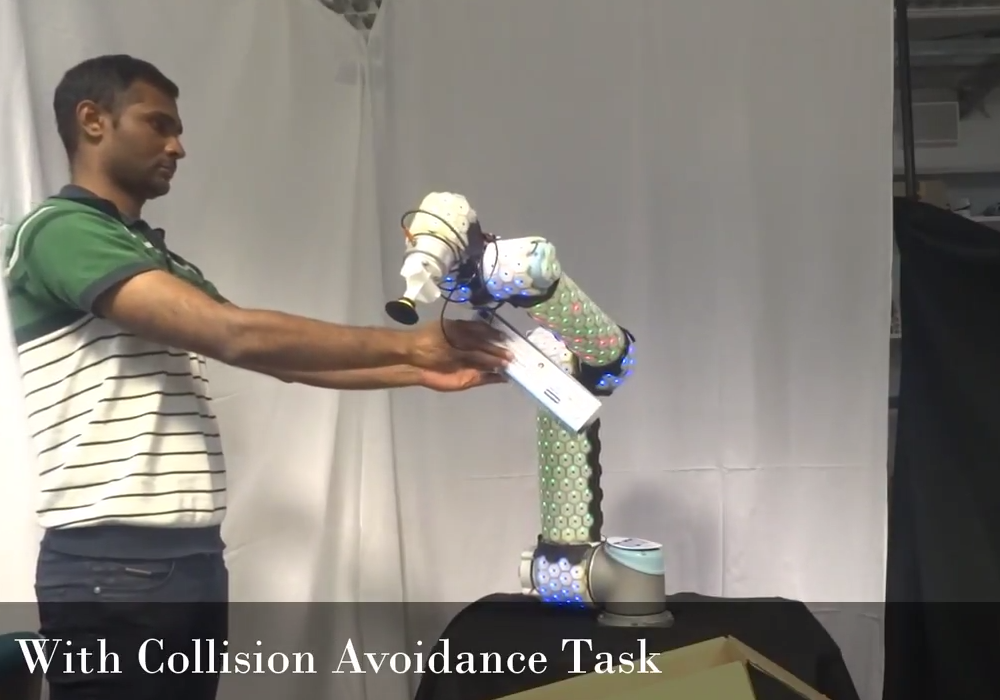
\includegraphics[width=6.5cm,height=6cm]{chapters/doa/images/delft/test_pick2place/cropped/test1_2_2-cropped.png}}
\end{subfigure}
\begin{subfigure}
[Final State - Place Position]{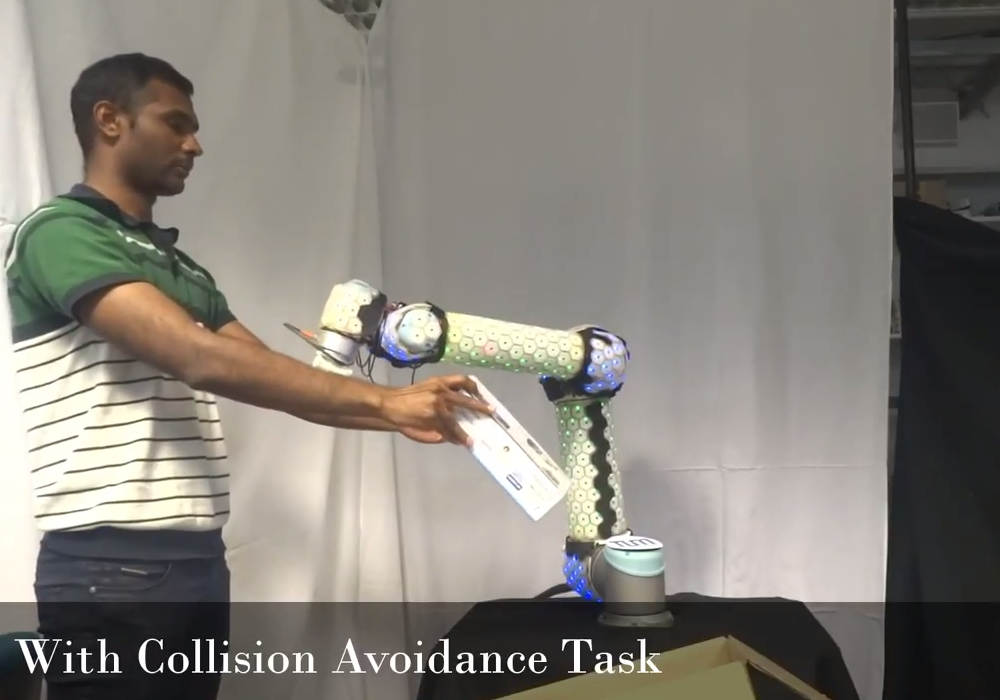
\includegraphics[width=6.5cm,height=6cm]{chapters/doa/images/delft/test_pick2place/cropped/test1_3-cropped.png}}
\end{subfigure}
\caption{Pick to Place Location: Test 2}
\label{fig:p2ptest2}
\end{figure}

\begin{figure}[H]
\centering
\begin{subfigure}
[Initial State - Pick Position]{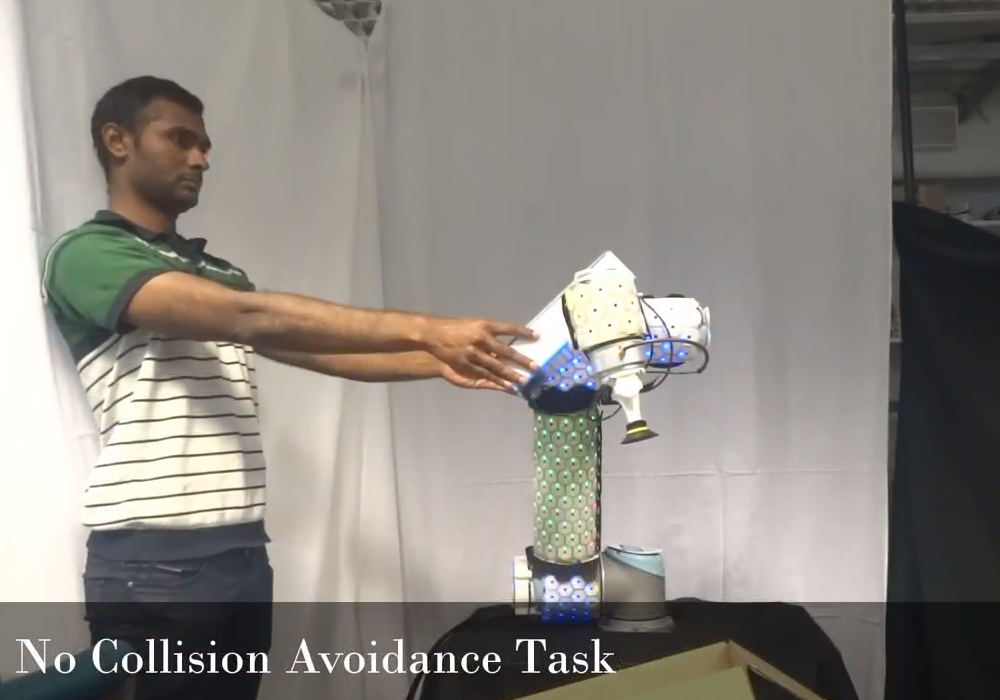
\includegraphics[width=6.5cm,height=6cm]{chapters/doa/images/delft/test_pick2place/cropped/test2_0-cropped.png}}
\end{subfigure}
\begin{subfigure}
[Colliding with Obstacle]{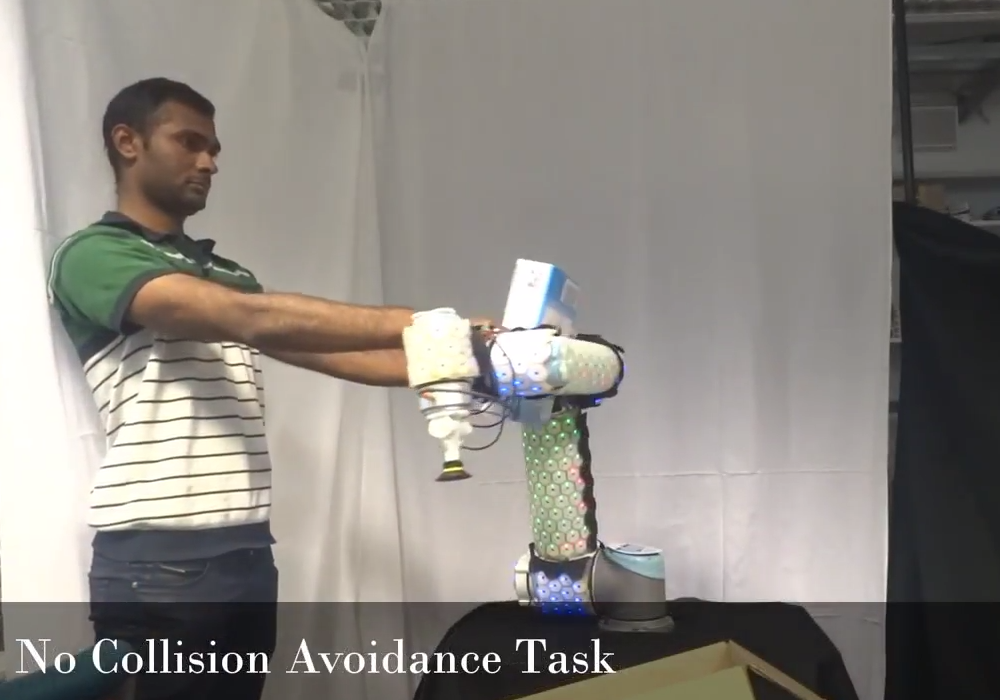
\includegraphics[width=6.5cm,height=6cm]{chapters/doa/images/delft/test_pick2place/cropped/test2_1-cropped.png}}
\end{subfigure}
\begin{subfigure}
[Avoiding Local Collisions 1/3]{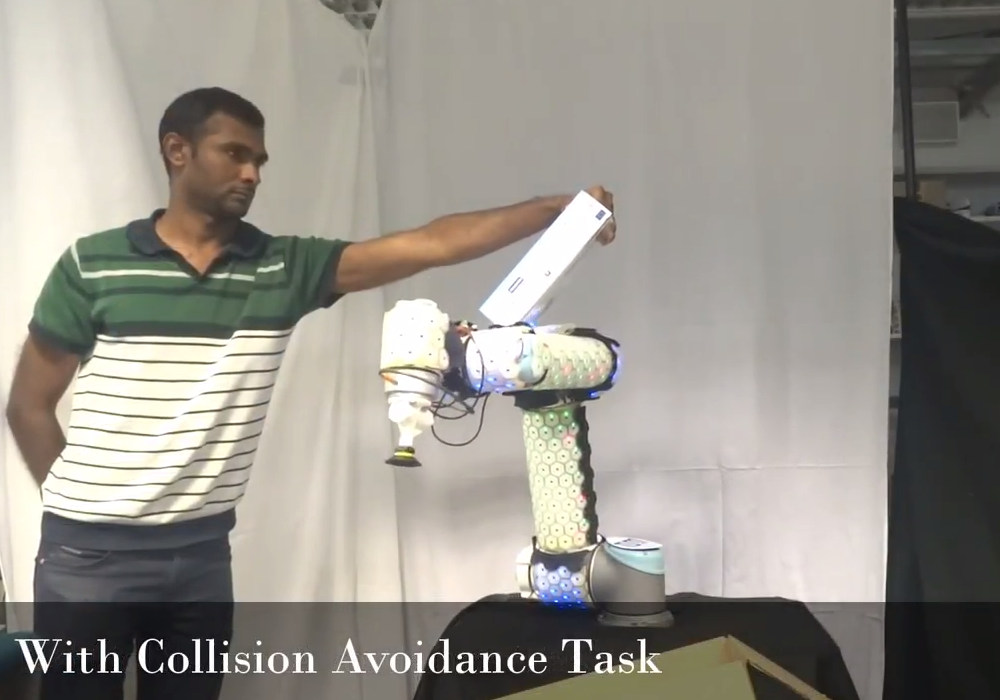
\includegraphics[width=6.5cm,height=6cm]{chapters/doa/images/delft/test_pick2place/cropped/test2_2-cropped.png}}
\end{subfigure}
\begin{subfigure}
[Avoiding Local Collisions 2/3]{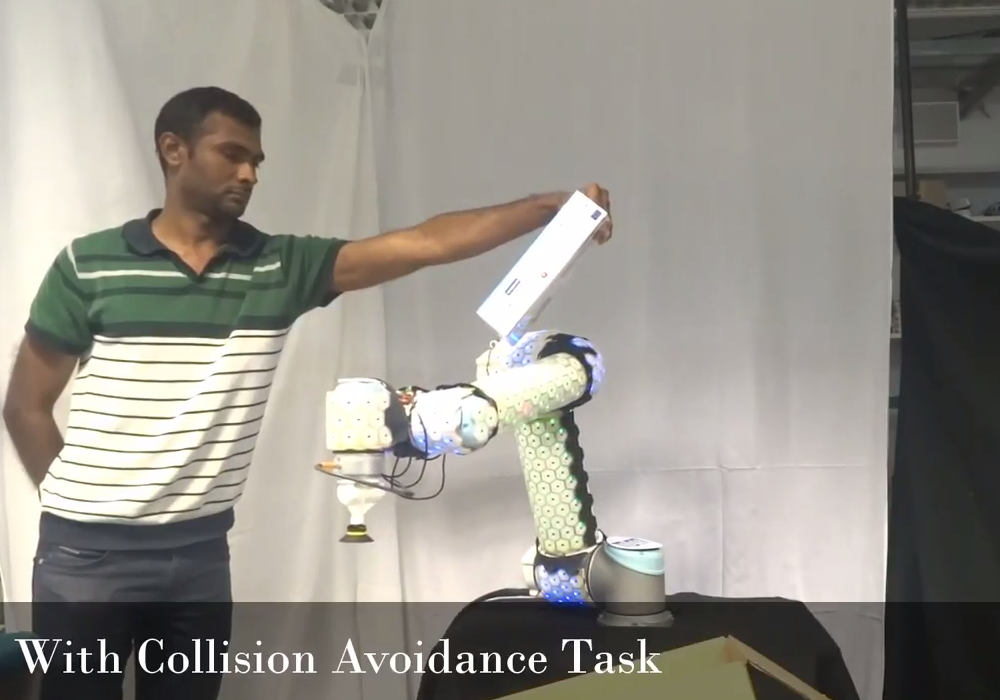
\includegraphics[width=6.5cm,height=6cm]{chapters/doa/images/delft/test_pick2place/cropped/test2_2_1-cropped.png}}
\end{subfigure}
\begin{subfigure}
[Avoiding Local Collisions 3/3]{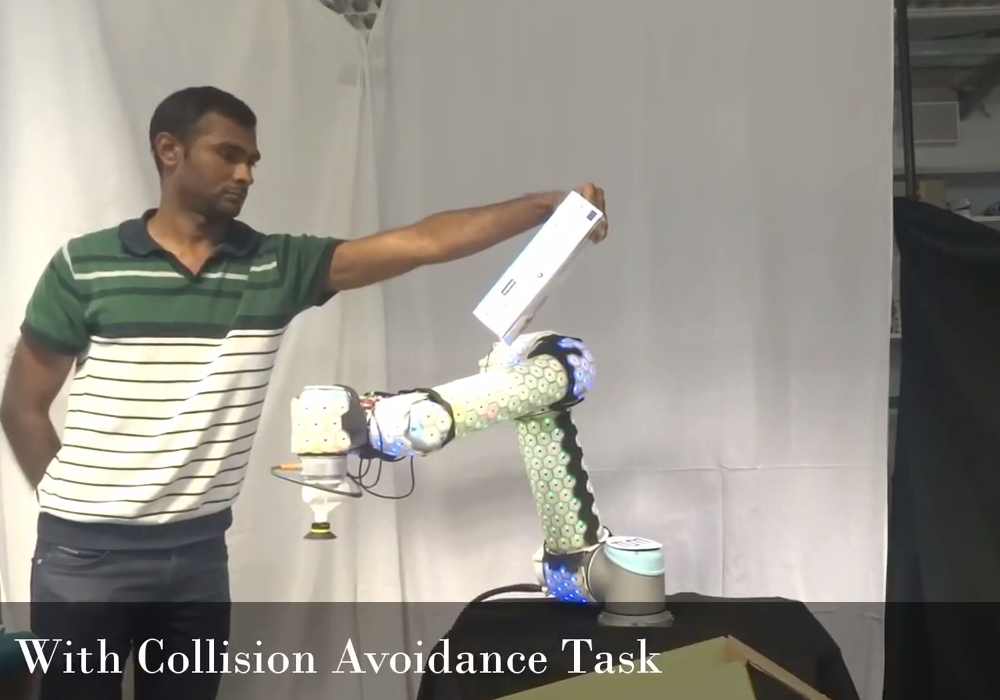
\includegraphics[width=6.5cm,height=6cm]{chapters/doa/images/delft/test_pick2place/cropped/test2_2_2-cropped.png}}
\end{subfigure}
\begin{subfigure}
[Final State - Place Position]{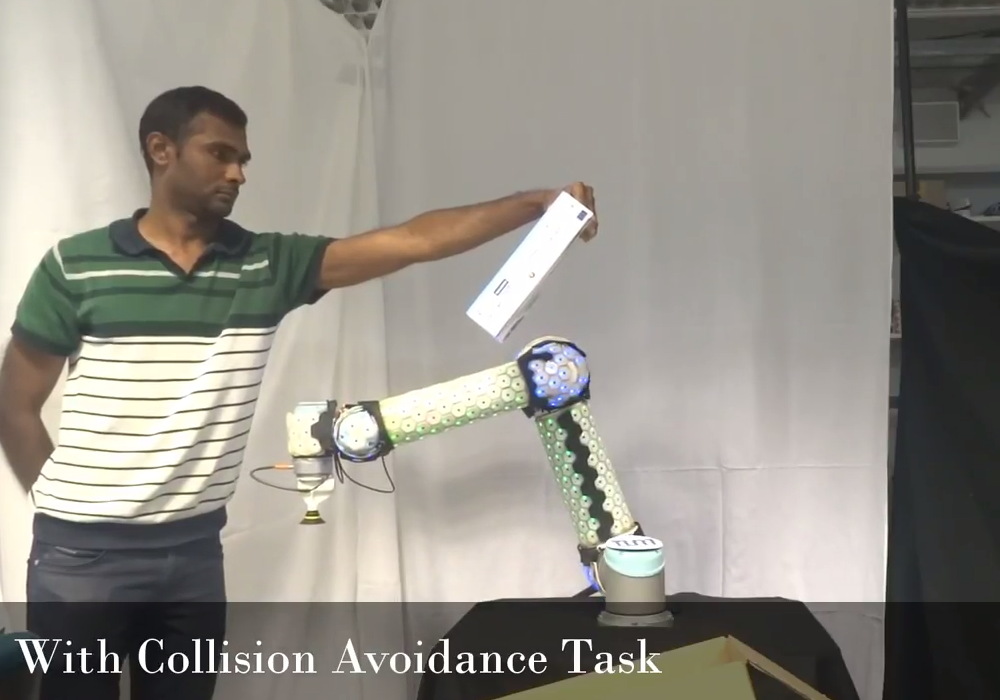
\includegraphics[width=6.5cm,height=6cm]{chapters/doa/images/delft/test_pick2place/cropped/test2_3-cropped.png}}
\end{subfigure}
\caption{Pick to Place Location: Test 3}
\label{fig:p2ptest3}
\end{figure}

\begin{figure}[H]
\centering
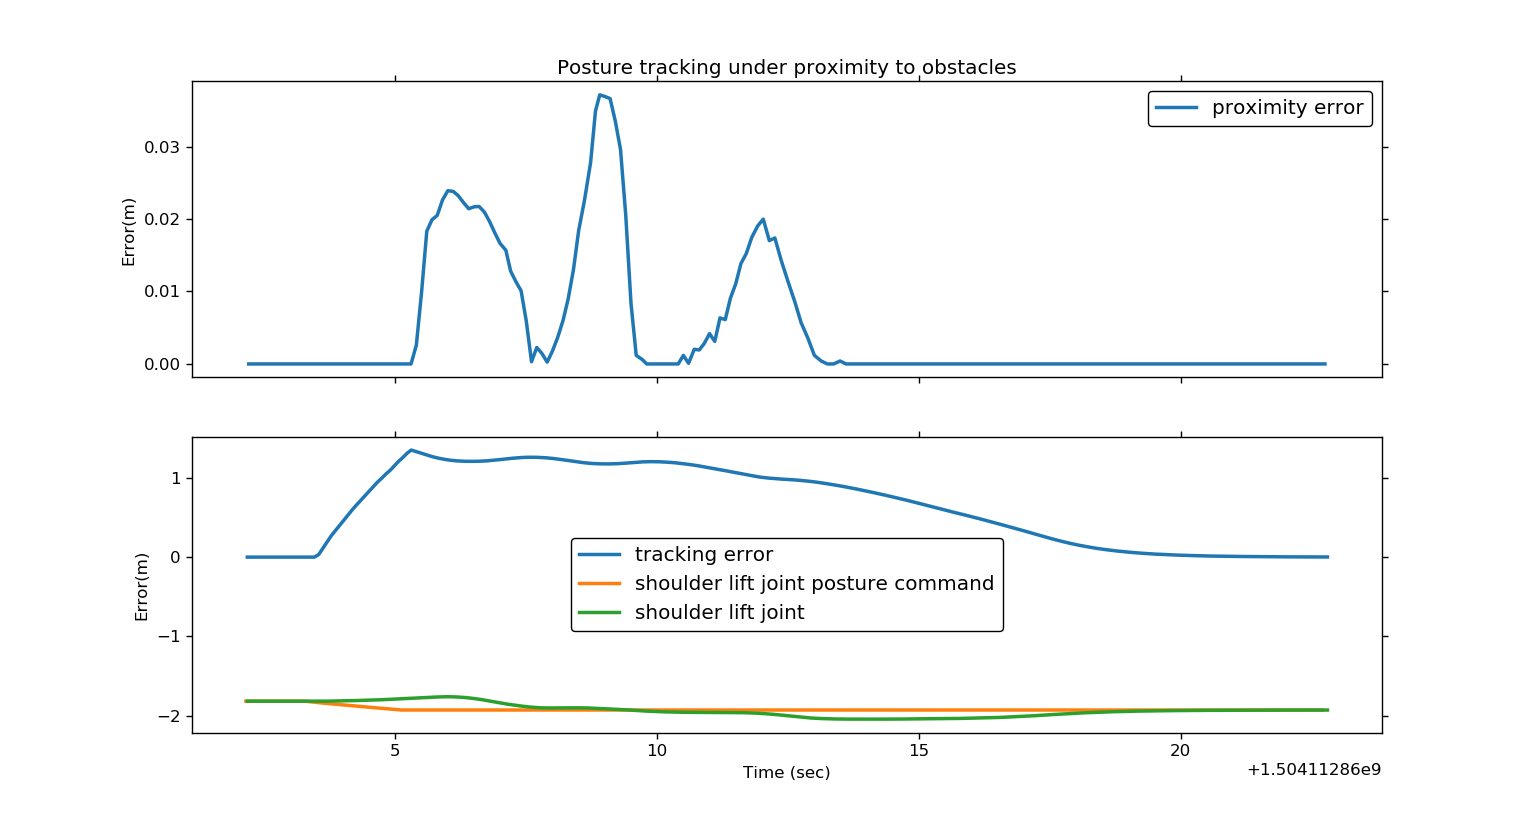
\includegraphics[width=15cm,height=6cm,center]{chapters/doa/images/delft/test_pick2place/test0.png}
\caption{Pick2Place: Posture/Proximity Error Evolution for Test 1}
\label{pick2place:test1}
\end{figure}

\begin{figure}[H]
\centering
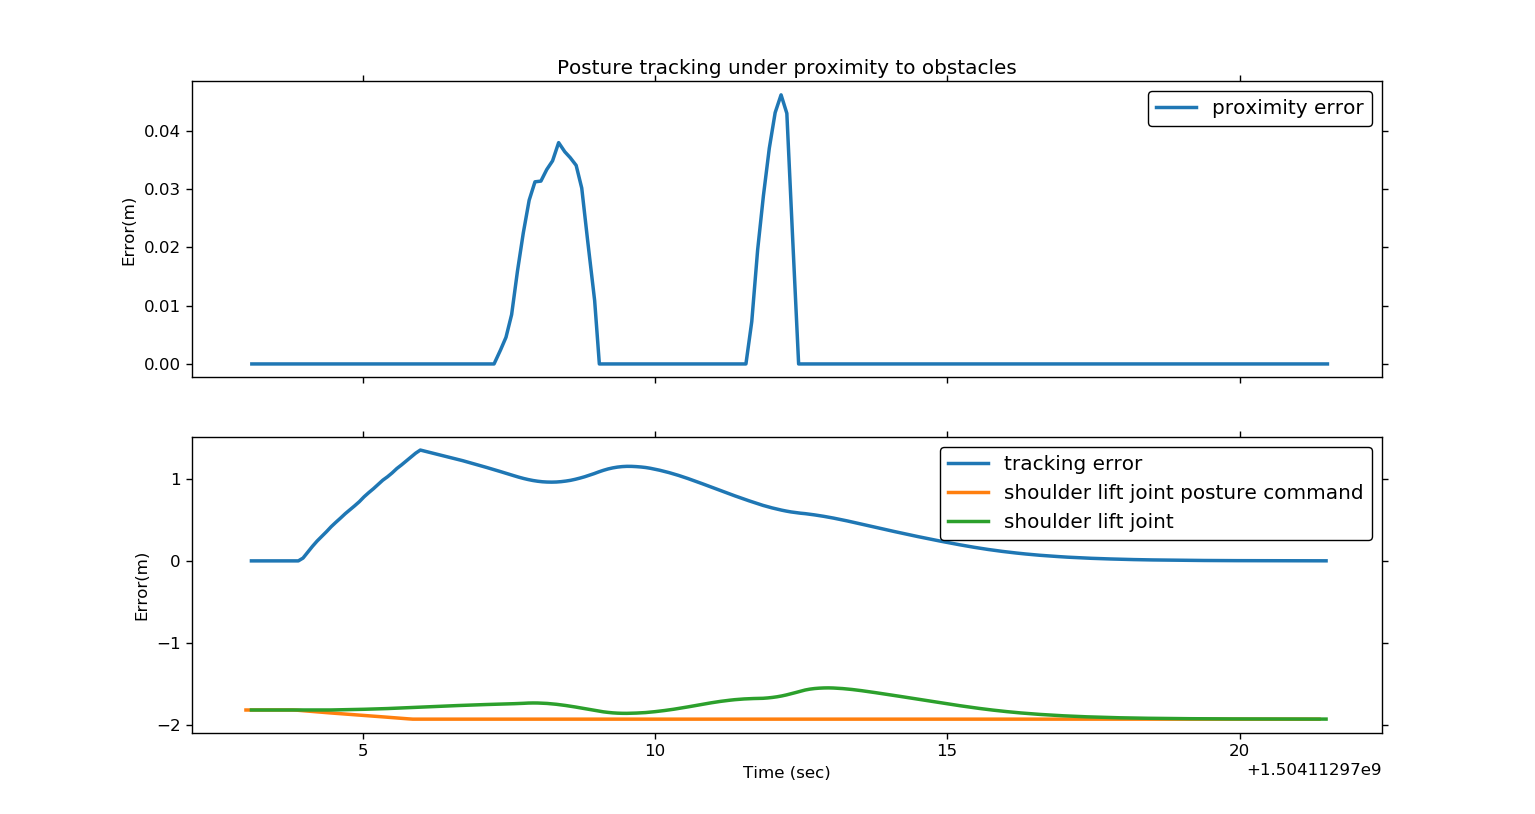
\includegraphics[width=15cm,height=6cm,center]{chapters/doa/images/delft/test_pick2place/test1.png}
\caption{Pick2Place: Posture/Proximity Error Evolution for Test 2}
\label{pick2place:test2}
\end{figure}

\begin{figure}[H]
\centering
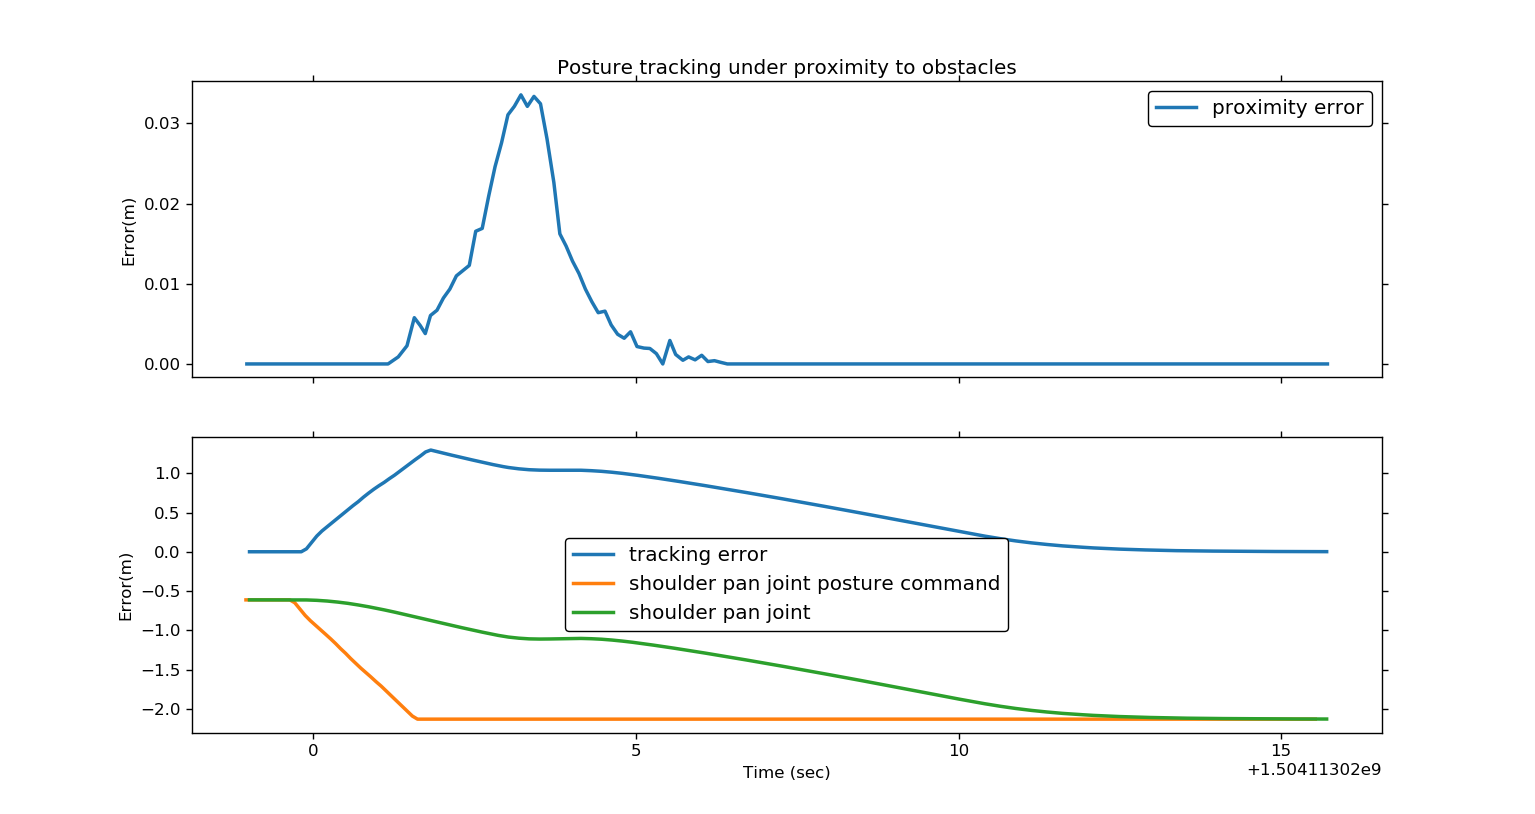
\includegraphics[width=15cm,height=6cm,center]{chapters/doa/images/delft/test_pick2place/test2.png}
\caption{Pick2Place: Posture/Proximity Error Evolution for Test 3}
\label{pick2place:test3}
\end{figure}
The figure \ref{fig:p2ptest2} shows the second test with a fixed obstacle location through out this test. (a) shows the initial state of the robot which is the home position and (b) shows the trajectory execution without any collision avoidance task to differentiate with the behavior generated by the controller with collision avoidance task. The robot evading collisions and its inability to reach the goal because of the object can be seen in (c), (d), (e) and (f). The figure \ref{fig:p2ptest3} shows the second test with a fixed obstacle location through out this test. (a) shows the initial state of the robot which is the home position and (b) shows the trajectory execution without any collision avoidance task to differentiate with the behavior generated by the controller with collision avoidance task. The robot evading collisions and its inability to reach the goal because of the object can be seen in (c), (d), (e) and (f). The plots \ref{pick2place:test1},\ref{pick2place:test2}, \ref{pick2place:test3} show the evolution of the trajectory tracking error with relevance to proximity error expressing the collision avoidance action in reality. The oscillations of the joint are lesser while tracking because of the smooth collision avoidance action as seen in the video. The shoulder pan and lift joint states are also plotted with the corresponding posture command to showing the nature of the trajectory tracking in these experiments.  
\begin{figure}[H]
\centering
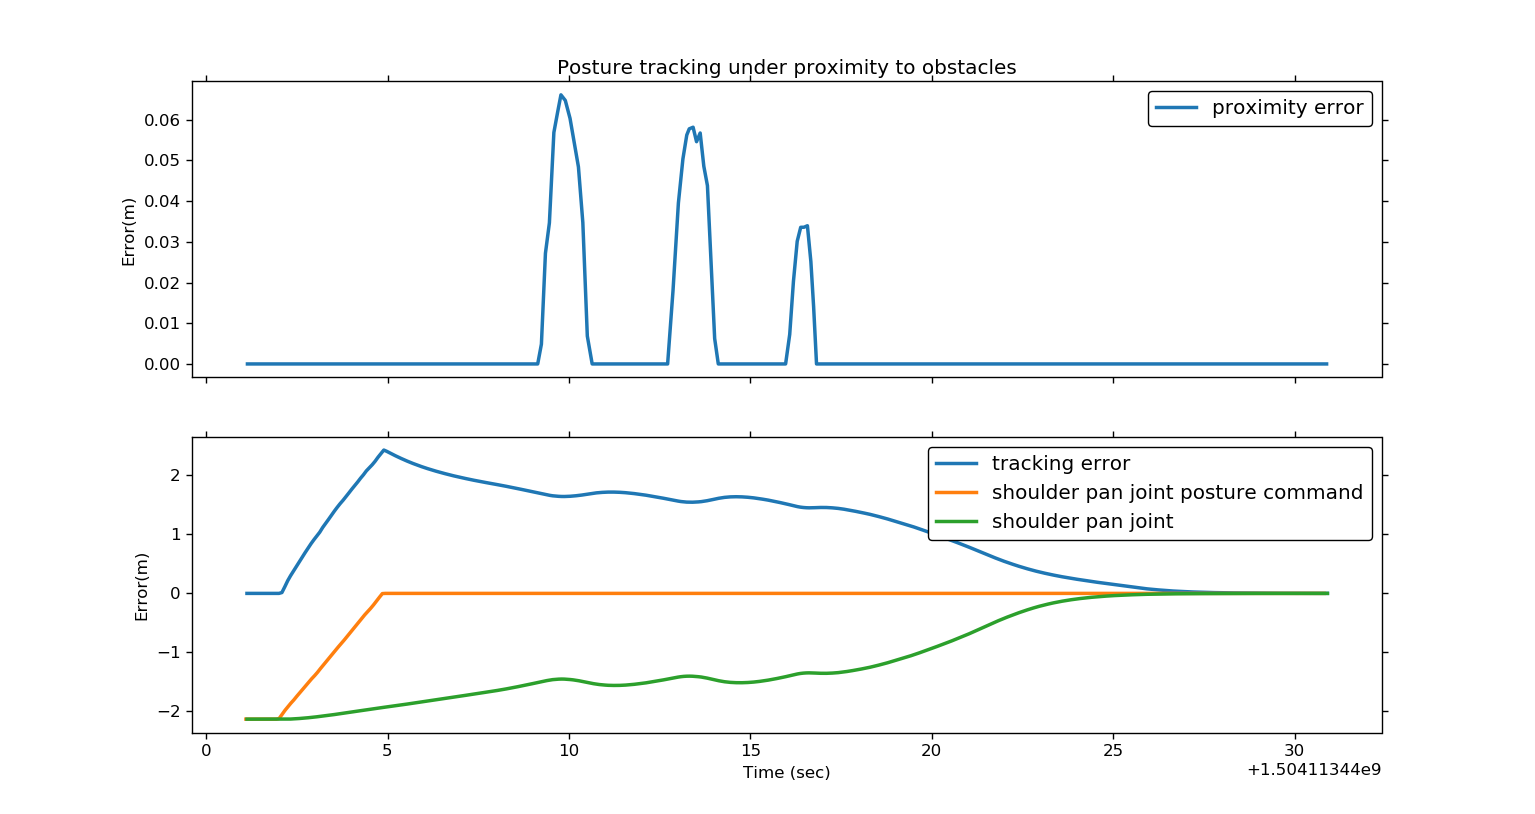
\includegraphics[width=15cm,height=6cm,center]{chapters/doa/images/delft/test_place2home/test1.png}
\caption{Place2Home: Posture/Proximity Error Evolution for Test 1}
\label{Place2Home:test1}
\end{figure}
\subsubsection{Place to Home}
The validation is shown in the \href{https://goo.gl/GP8KAA}{\textcolor{blue}{place to home}} experiment video
The figure \ref{fig:p2htest1} shows the second test with a fixed obstacle location through out this test. (a) shows the initial state of the robot which is the home position and (b) shows the trajectory execution without any collision avoidance task to differentiate with the behavior generated by the controller with collision avoidance task. The robot evading collisions and its inability to reach the goal because of the object can be seen in (c) and (d). 

The figure \ref{fig:p2htest2} shows the second test with a fixed obstacle location through out this test. (a) shows the initial state of the robot which is the home position and (b) shows the trajectory execution without any collision avoidance task to differentiate with the behavior generated by the controller with collision avoidance task. The robot evading collisions and its inability to reach the goal because of the object can be seen in (c) and (d). 

The figure \ref{fig:p2htest3} shows the third test with a fixed obstacle location through out this test. (a) shows the initial state of the robot which is the home position and (b) shows the trajectory execution without any collision avoidance task to differentiate with the behavior generated by the controller with collision avoidance task. The robot evading collisions and its inability to reach the goal because of the object can be seen in (c) and (d). The plots \ref{Place2Home:test1},\ref{Place2Home:test2} show the evolution of the trajectory tracking error with relevance to proximity error expressing the collision avoidance action in reality.

\begin{figure}[H]
\centering
\begin{subfigure}
[Initial State - Place Position]{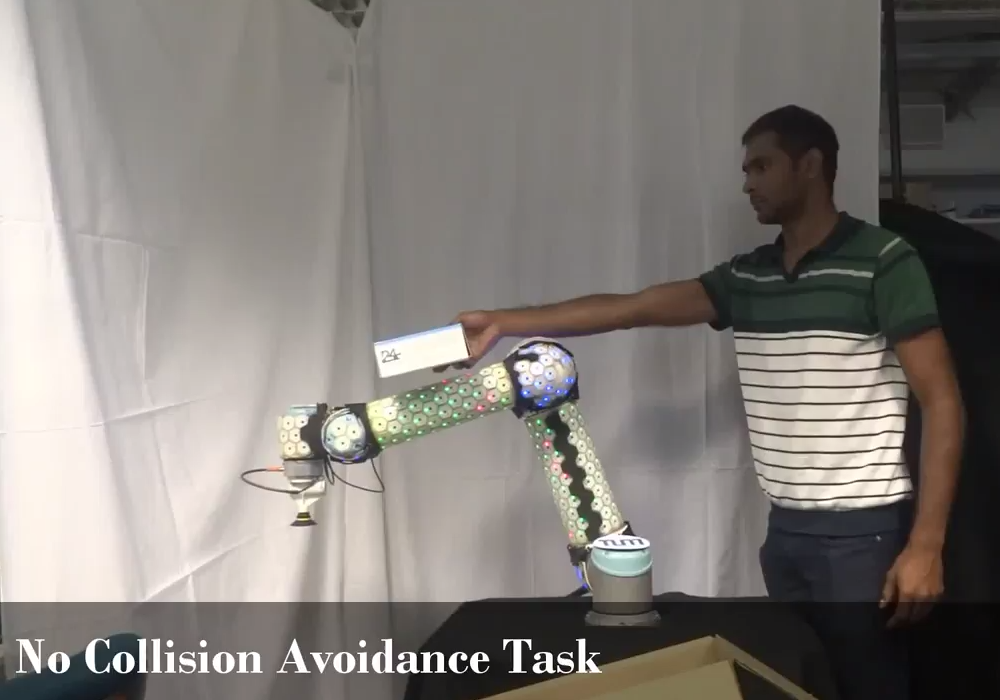
\includegraphics[width=6.5cm,height=6cm]{chapters/doa/images/delft/test_place2home/cropped/test0_0-cropped.png}}
\end{subfigure}
\begin{subfigure}
[Colliding with Obstacle]{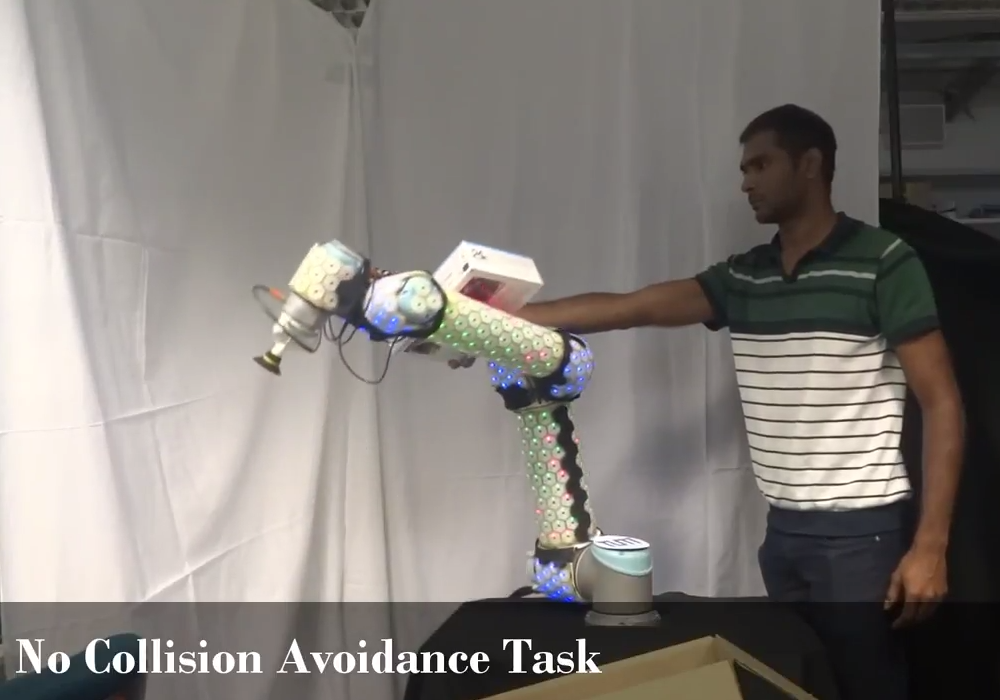
\includegraphics[width=6.5cm,height=6cm]{chapters/doa/images/delft/test_place2home/cropped/test0_1-cropped.png}}
\end{subfigure}
\begin{subfigure}
[Avoiding Local Collisions 1/3]{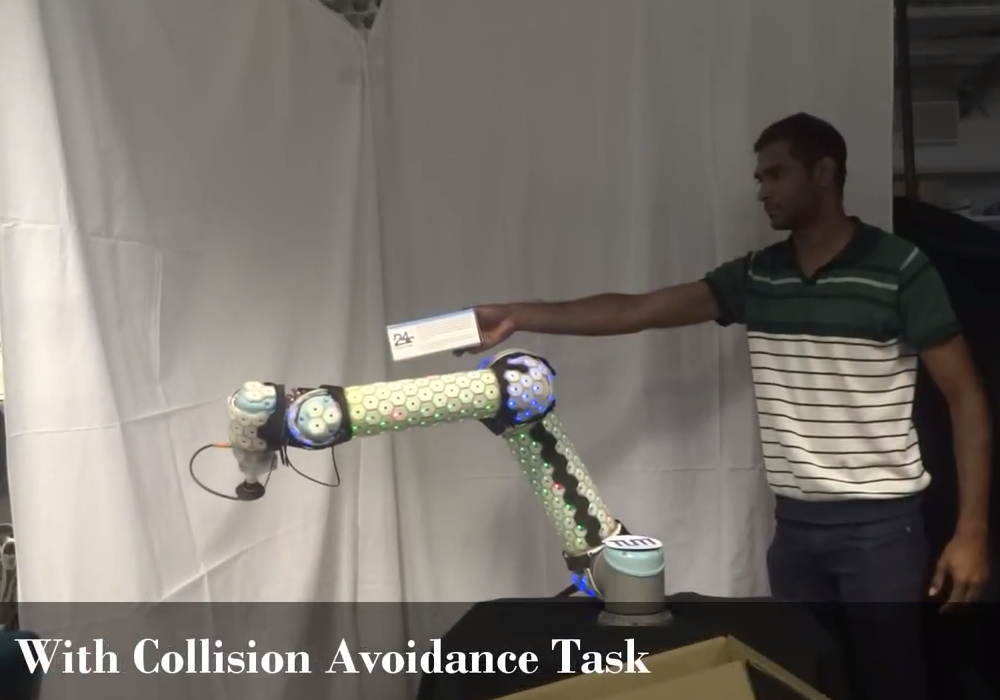
\includegraphics[width=6.5cm,height=6cm]{chapters/doa/images/delft/test_place2home/cropped/test0_2-cropped.png}}
\end{subfigure}
\begin{subfigure}
[Avoiding Local Collisions 2/3]{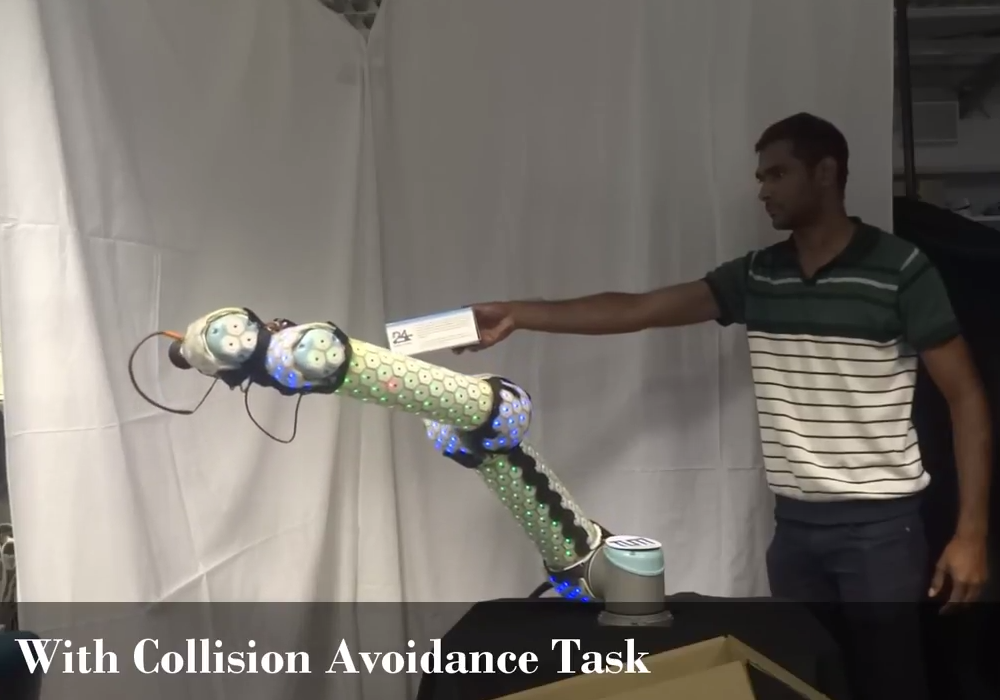
\includegraphics[width=6.5cm,height=6cm]{chapters/doa/images/delft/test_place2home/cropped/test0_3-cropped.png}}
\end{subfigure}
\begin{subfigure}
[Avoiding Local Collisions 3/3]{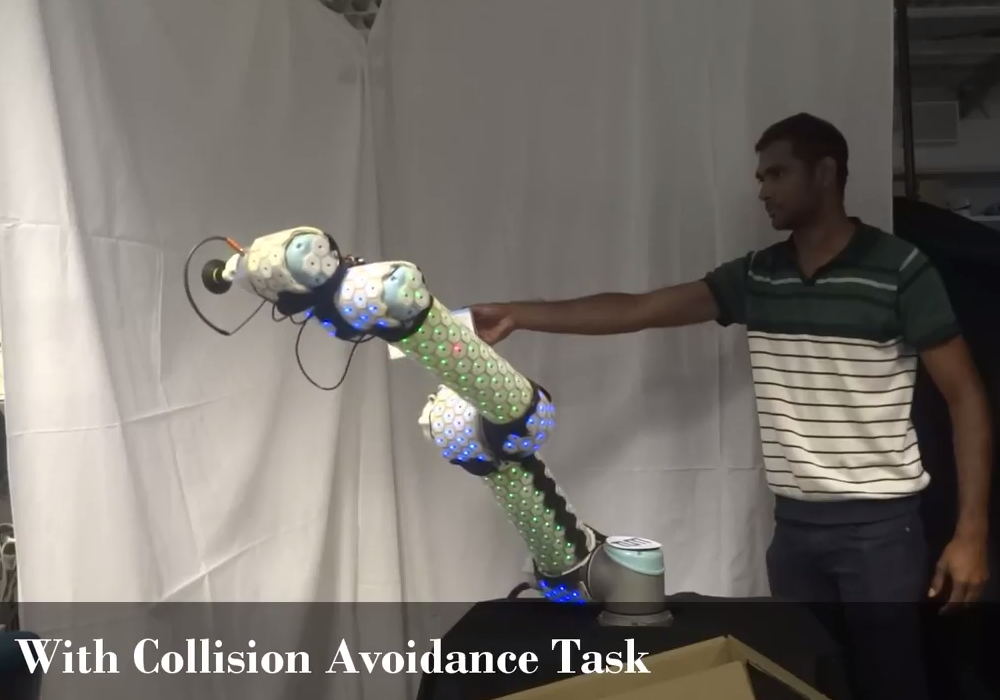
\includegraphics[width=6.5cm,height=6cm]{chapters/doa/images/delft/test_place2home/cropped/test0_x-cropped.png}}
\end{subfigure}
\begin{subfigure}
[Reaching Final State - Home Position]{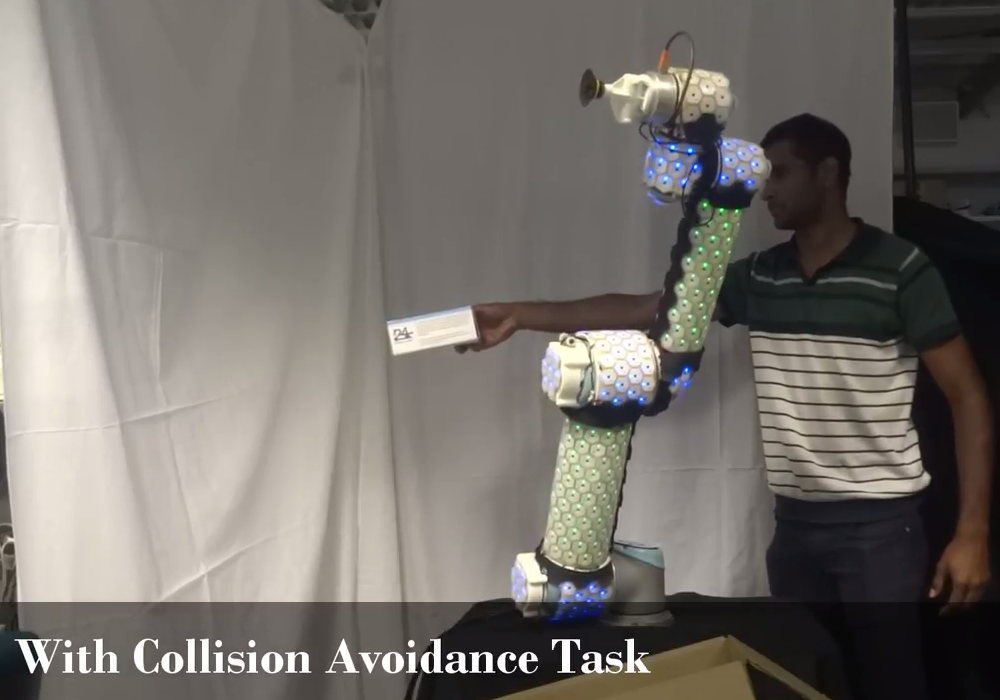
\includegraphics[width=6.5cm,height=6cm]{chapters/doa/images/delft/test_place2home/cropped/test0_4-cropped.png}}
\end{subfigure}
\caption{Place to Home Location: Test 1}
\label{fig:p2htest1}
\end{figure}

\begin{figure}[H]
\centering
\begin{subfigure}
[Initial State - Home Position]{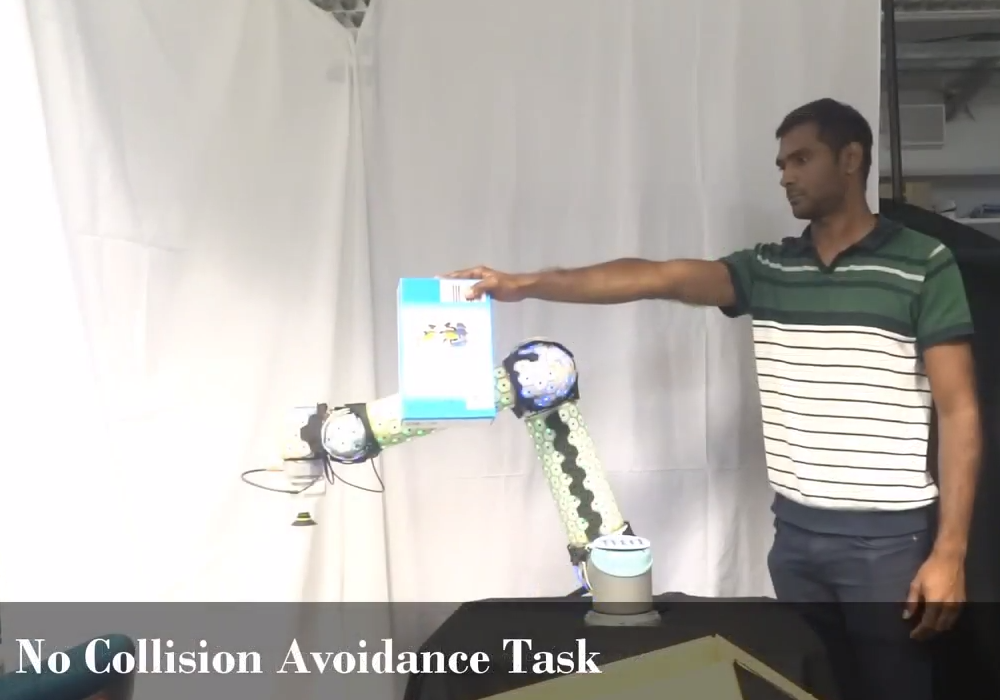
\includegraphics[width=6.5cm,height=6cm]{chapters/doa/images/delft/test_place2home/cropped/test1_0-cropped.png}}
\end{subfigure}
\begin{subfigure}
[Colliding with Obstacle]{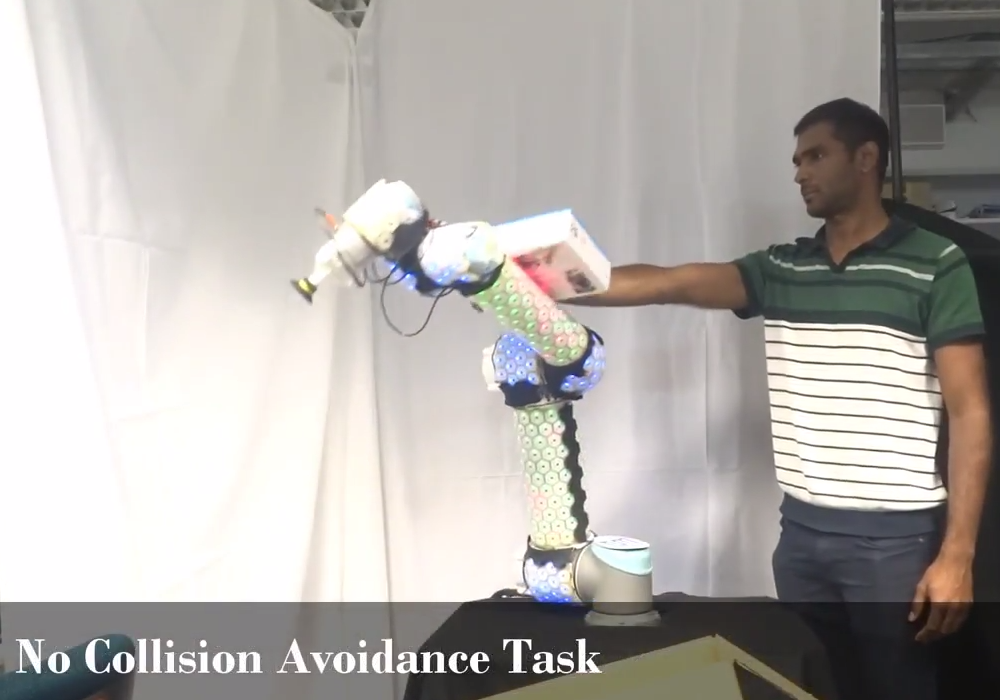
\includegraphics[width=6.5cm,height=6cm]{chapters/doa/images/delft/test_place2home/cropped/test1_1-cropped.png}}
\end{subfigure}
\begin{subfigure}
[Avoiding Local Collisions 1/3]{\includegraphics[width=6.5cm,height=6cm]{chapters/doa/images/delft/test_place2home/cropped/test1_2-cropped.png}}
\end{subfigure}
\begin{subfigure}
[Avoiding Local Collisions 2/3]{\includegraphics[width=6.5cm,height=6cm]{chapters/doa/images/delft/test_place2home/cropped/test1_3-cropped.png}}
\end{subfigure}
\begin{subfigure}
[Avoiding Local Collisions 3/3]{\includegraphics[width=6.5cm,height=6cm]{chapters/doa/images/delft/test_place2home/cropped/test1_x-cropped.png}}
\end{subfigure}
\begin{subfigure}
[Final State - Place Position]{\includegraphics[width=6.5cm,height=6cm]{chapters/doa/images/delft/test_place2home/cropped/test1_4-cropped.png}}
\end{subfigure}
\caption{Place to Home Location: Test 2}
\label{fig:p2htest2}
\end{figure}
\begin{figure}[H]
\centering
\begin{subfigure}
[Initial State - Home Position]{\includegraphics[width=6.5cm,height=6cm]{chapters/doa/images/delft/test_place2home/cropped/test2_0-cropped.png}}
\end{subfigure}
\begin{subfigure}
[Colliding with Obstacle]{\includegraphics[width=6.5cm,height=6cm]{chapters/doa/images/delft/test_place2home/cropped/test2_1-cropped.png}}
\end{subfigure}
\begin{subfigure}
[Avoiding Local Collisions 1/3]{\includegraphics[width=6.5cm,height=6cm]{chapters/doa/images/delft/test_place2home/cropped/test2_2-cropped.png}}
\end{subfigure}
\begin{subfigure}
[Avoiding Local Collisions 2/3]{\includegraphics[width=6.5cm,height=6cm]{chapters/doa/images/delft/test_place2home/cropped/test2_3-cropped.png}}
\end{subfigure}
\begin{subfigure}
[Avoiding Local Collisions 3/3]{\includegraphics[width=6.5cm,height=6cm]{chapters/doa/images/delft/test_place2home/cropped/test2_4-cropped.png}}
\end{subfigure}
\begin{subfigure}
[Final State - Place Position]{\includegraphics[width=6.5cm,height=6cm]{chapters/doa/images/delft/test_place2home/cropped/test2_5-cropped.png}}
\end{subfigure}
\caption{Place to Home Location: Test 3}
\label{fig:p2htest3}
\end{figure}
\begin{figure}[H]
\centering
\includegraphics[width=15cm,height=6cm,center]{chapters/doa/images/delft/test_place2home/test2.png}
\caption{Place2Home: Posture/Proximity Error Evolution for Test 1}
\label{Place2Home:test2}
\end{figure}
   

\subsubsection{Complete Manipulation Scenario}
The reactive collision avoidance component is applied on a complete manipulation scenario involving multiple sequences of pick and place operations using a suction gripper in the end effector. The controller still holds the same ring of collision constraints in the upper arm. The demonstration video is shown in this link https://goo.gl/PLbKdb. It can be observed that the behavior is very reactive after proper tuning of the controller and the task gains.    